% Copyright 2004 by Till Tantau <tantau@users.sourceforge.net>.
%
% In principle, this file can be redistributed and/or modified under
% the terms of the GNU Public License, version 2.
%
% However, this file is supposed to be a template to be modified
% for your own needs. For this reason, if you use this file as a
% template and not specifically distribute it as part of a another
% package/program, I grant the extra permission to freely copy and
% modify this file as you see fit and even to delete this copyright
% notice.

\documentclass{beamer}

% There are many different themes available for Beamer. A comprehensive
% list with examples is given here:
% http://deic.uab.es/~iblanes/beamer_gallery/index_by_theme.html
% You can uncomment the themes below if you would like to use a different
% one:
%\usetheme{AnnArbor}
%\usetheme{Antibes}
%\usetheme{Bergen}
%\usetheme{Berkeley}
%\usetheme{Berlin}
% \usetheme{Boadilla}
%\usetheme{boxes}
%\usetheme{CambridgeUS}
%\usetheme{Copenhagen}
%\usetheme{Darmstadt}
%\usetheme{default}
%\usetheme{Frankfurt}
%\usetheme{Goettingen}
%\usetheme{Hannover}
%\usetheme{Ilmenau}
%\usetheme{JuanLesPins}
%\usetheme{Luebeck}
\usetheme{Madrid}
%\usetheme{Malmoe}
%\usetheme{Marburg}
%\usetheme{Montpellier}
%\usetheme{PaloAlto}
%\usetheme{Pittsburgh}
%\usetheme{Rochester}
%\usetheme{Singapore}
%\usetheme{Szeged}
%\usetheme{Warsaw}

% Modifying footline
\setbeamertemplate{navigation symbols}{}
\makeatother
\setbeamertemplate{footline}
{
  \leavevmode%
  \hbox{%
  \begin{beamercolorbox}[wd=.5\paperwidth,ht=2.25ex,dp=1ex,center]{author in head/foot}%
    \usebeamerfont{author in head/foot}\insertshortauthor
  \end{beamercolorbox}%
  \begin{beamercolorbox}[wd=.5\paperwidth,ht=2.25ex,dp=1ex,center]{title in head/foot}%
    \usebeamerfont{title in head/foot}\insertshorttitle\hspace*{3em}
    \insertframenumber{} / \inserttotalframenumber\hspace*{1ex}
  \end{beamercolorbox}}%
  \vskip0pt%
}
\makeatletter
\setbeamertemplate{navigation symbols}{}

\usepackage{amsthm}
\usepackage{amsmath}
\usepackage{amsfonts}
\usepackage{amssymb}

% Bold shortcuts
\newcommand{\bb}[1]{\mathbf{#1}}
% - lowercase
\newcommand{\bbb}{\bb{b}}
\newcommand{\bx}{\bb{x}}
\newcommand{\bxi}{\bx^{(i)}}
\newcommand{\bxl}{\bx^{(l)}}
\newcommand{\bt}{\bb{t}}
\newcommand{\by}{\bb{y}}
\newcommand{\bv}{\bb{v}}
\newcommand{\bw}{\bb{w}}
\newcommand{\bc}{\bb{c}}
\newcommand{\bd}{\bb{d}}
\newcommand{\bg}{\bb{g}}
\newcommand{\bh}{\bb{h}}
\newcommand{\br}{\bb{r}}
\newcommand{\bu}{\bb{u}}
\newcommand{\byl}{\by^{(l)}}
\newcommand{\bz}{\bb{z}}
\newcommand{\bzi}{\bz^{(i)}}
\newcommand{\bzl}{\bz^{(l)}}
\newcommand{\bzil}{\bz^{(i,l)}}
\newcommand{\bpa}{\bb{pa}}

\newcommand{\bT}{\boldsymbol{\theta}}
\newcommand{\bTl}{\boldsymbol{\theta}^{(l)}}
\newcommand{\balpha}{\boldsymbol{\alpha}}
\newcommand{\bphi}{\boldsymbol{\phi}}
\newcommand{\beps}{\boldsymbol{\epsilon}}
\newcommand{\bepsl}{\beps^{(l)}}
\newcommand{\bepsil}{\beps^{(i,l)}}
\newcommand{\bzeta}{\boldsymbol{\zeta}}
\newcommand{\bzetal}{\zeta^{(l)}}
\newcommand{\bsigma}{\boldsymbol{\sigma}}
\newcommand{\bmu}{\boldsymbol{\mu}}
\newcommand{\bzero}{\bb{0}}

% - uppercase
\newcommand{\bL}{\bb{L}}
\newcommand{\bV}{\bb{V}}
\newcommand{\bW}{\bb{W}}
\newcommand{\bI}{\bb{I}}
\newcommand{\bR}{\bb{R}}
\newcommand{\bX}{\bb{X}}
\newcommand{\bO}{\bb{O}}

\newcommand{\btPa}{\widetilde{\bb{Pa}}}
\newcommand{\btpa}{\widetilde{\bb{pa}}}

% Tilde
\newcommand{\tz}{\widetilde{z}}
\newcommand{\tZ}{\widetilde{Z}}
\newcommand{\tf}{\widetilde{f}}
\newcommand{\btZ}{\widetilde{\bb{Z}}}
\newcommand{\btz}{\widetilde{\bz}}
\newcommand{\btT}{\widetilde{\bT}}
\newcommand{\tPa}{\widetilde{Pa}}

\newcommand{\pT}{p_{\bT}}
\newcommand{\pTl}{p_{\bT^{(l)}}}
\newcommand{\pA}{p_{\balpha}}
\newcommand{\qT}{q_{\bT}}
\newcommand{\qPhi}{q_{\bphi}}
\newcommand{\fT}{f_{\bT}}
\newcommand{\fPhi}{f_{\bphi}}
\newcommand{\fTPhi}{f_{\bT,\bphi}}
\newcommand{\gT}{g_{\bT}}
\newcommand{\gPhi}{g_{\bphi}}
\newcommand{\hPhi}{h_{\bphi}}

\newcommand{\Exp}[2]{\mathbb{E}_{#1}\left[#2\right]}
\newcommand{\Ed}{\mathbb{E}_\bd}
\newcommand{\eqnr}{\addtocounter{equation}{1}\tag{\theequation}}

\DeclareMathOperator*{\argmax}{argmax}

% Create 'example' environment
\theoremstyle{definition}
\newtheorem{exmp}{Example}[section]

% Variational bound
\newcommand{\LB}[2]{\mathcal{L}^{#1}(\bT,\bphi; #2)}
\newcommand{\LBT}[2]{\widetilde{\mathcal{L}}^{#1}(\bT,\bphi; #2)}


\usepackage{tikz}
\usetikzlibrary{decorations.pathmorphing, patterns,shapes}
\usetikzlibrary{arrows.meta}
\usetikzlibrary{bayesnet}

\usepackage{algorithm}
\usepackage[noend]{algpseudocode}

\usepackage{color}

\title{Auto-Encoding Variational Bayes}
\subtitle{Diederik P. Kingma and Max Welling}

% A subtitle is optional and this may be deleted
% \subtitle{Optional Subtitle}

\author{Ashish Bora}

% - Give the names in the same order as the appear in the paper.
% - Use the \inst{?} command only if the authors have different
%   affiliation.

% - Use the \inst command only if there are several affiliations.
% - Keep it simple, no one is interested in your street address.

\date{Oct 2016}
% - Either use conference name or its abbreviation.
% - Not really informative to the audience, more for people (including
%   yourself) who are reading the slides online

% \subject{Theoretical Computer Science}
% This is only inserted into the PDF information catalog. Can be left
% out.

% If you have a file called "university-logo-filename.xxx", where xxx
% is a graphic format that can be processed by latex or pdflatex,
% resp., then you can add a logo as follows:

% \pgfdeclareimage[height=0.5cm]{university-logo}{university-logo-filename}
% \logo{\pgfuseimage{university-logo}}

% Delete this, if you do not want the table of contents to pop up at
% the beginning of each subsection:
\AtBeginSubsection[]
{
  \begin{frame}<beamer>{Outline}
    \tableofcontents[currentsection,currentsubsection]
  \end{frame}
}

% Let's get started
\begin{document}

\begin{frame}
  \titlepage
\end{frame}

\begin{frame}{Outline}
  \tableofcontents
  % You might wish to add the option [pausesections]
\end{frame}

% Section and subsections will appear in the presentation overview
% and table of contents.
\section{Quick intro to Bayesian Learning}

% \begin{frame}{Bayesian Learning}{}
%     \begin{figure}
%         \centering
%         \includegraphics[width=\textwidth]{evolution_bayes}
%     \end{figure}
%     Image taken from Google Images
% \end{frame}


\begin{frame}{Bayesian Learning}{}
    \begin{itemize}
        \item Observations $x$, Parameters/Unobserved variables $z$ \\
        Example
    \end{itemize}

    \begin{figure}
        \centering
        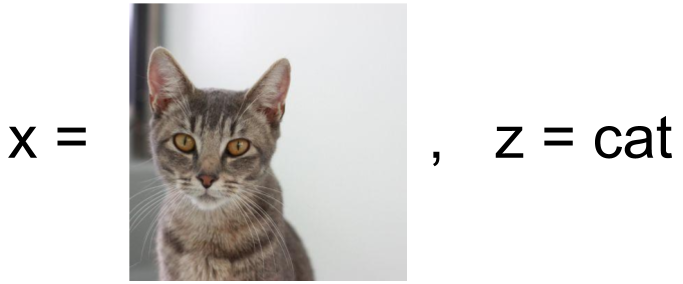
\includegraphics[width=0.6\textwidth]{bayes1}
    \end{figure}
    {\small Image from Google Images}
\end{frame}

\begin{frame}{Bayesian Learning}{}
    \begin{itemize}
        \item Observations $x$, Parameters/Unobserved variables $z$
        \item Likelihood = $p ( x \mid z )$
    \end{itemize}

    \begin{figure}
        \centering
        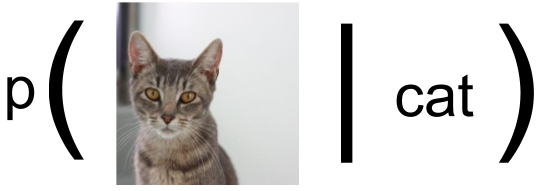
\includegraphics[width=0.6\textwidth]{bayes2}
    \end{figure}
    {\small Image from Google Images}
\end{frame}


\begin{frame}{Bayesian Learning}{}
    \begin{itemize}
        \item Observations $x$, Parameters/Unobserved variables $z$
        \item Likelihood = $p ( x \mid z )$
        \item Prior = $p ( z )$
    \end{itemize}

    \centering
    {\Huge p(cat)}

\end{frame}


\begin{frame}{Bayesian Learning}{}
    \begin{itemize}
        \item Observations $x$, Parameters/Unobserved variables $z$
        \item Likelihood = $p ( x \mid z )$
        \item Prior = $p ( z )$
        \item Joint = $p(x, z) = p(x \mid z) p(z)$
    \end{itemize}

    \begin{figure}
        \centering
        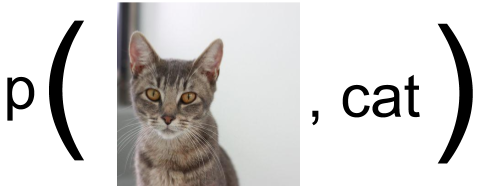
\includegraphics[width=0.6\textwidth]{bayes3}
    \end{figure}
    {\small Image from Google Images}
\end{frame}


\begin{frame}{Bayesian Learning}{}
    \begin{itemize}
        \item Observations $x$, Parameters/Unobserved variables $z$
        \item Likelihood = $p ( x \mid z )$
        \item Prior = $p ( z )$
        \item Joint = $p(x, z) = p(x \mid z) p(z)$
        \item Marginal Likelihood = $p(x) = \int_{z} p(x \mid z) p(z) dz$
    \end{itemize}

    \begin{figure}
        \centering
        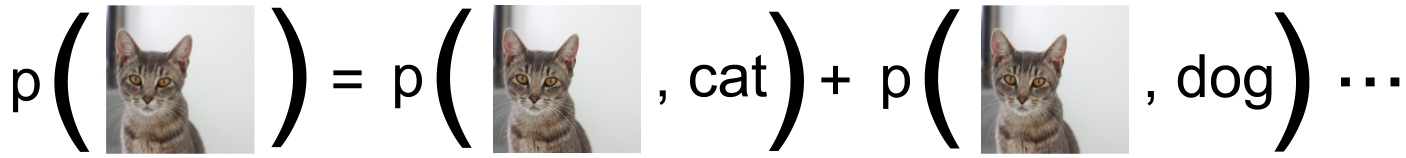
\includegraphics[width=\textwidth]{bayes4}
    \end{figure}
    {\small Image from Google Images}
\end{frame}


\begin{frame}{Bayesian Learning}{}
    \begin{itemize}
        \item Observations $x$, Parameters/Unobserved variables $z$
        \item Likelihood = $p ( x \mid z )$
        \item Prior = $p ( z )$
        \item Joint = $p(x, z) = p(x \mid z) p(z)$
        \item Marginal Likelihood = $p(x) = \int_{z} p(x \mid z) p(z) dz$
        \item Posterior = $p(z \mid x) $
    \end{itemize}

    \begin{figure}
        \centering
        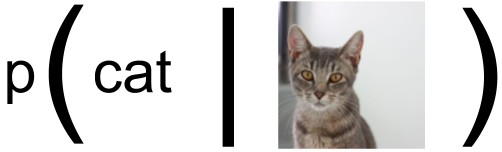
\includegraphics[width=0.5\textwidth]{bayes5}
    \end{figure}
    {\small Image from Google Images}
\end{frame}


\begin{frame}{Bayesian Learning}{}
    \begin{itemize}
        \item Observations $x$, Parameters/Unobserved variables $z$
        \item Likelihood = $p ( x \mid z )$
        \item Prior = $p ( z )$
        \item Joint = $p(x, z) = p(x \mid z) p(z)$
        \item Marginal Likelihood = $p(x) = \int_{z} p(x \mid z) p(z) dz$
        \item Posterior = $p(z \mid x) $
        \item {
            Non-Bayesian Learning : Maximize likelihood wrt parameters $z$ $$p ( x \mid z )$$
        }
        \item {
            Bayesian Learning : Maximize marginal likelihood with a prior $p(z)$ on parameters $z$ $$p(x)$$
        }
    \end{itemize}
\end{frame}


\section{Latent Variable Models}

\begin{frame}{Latent Variable Models}{}
    \begin{itemize}
        \item{
            Parameters: $\theta$, Latent variables: $z$, Observations $x$
        }
        \item{
            Two step process:
            \begin{center}
                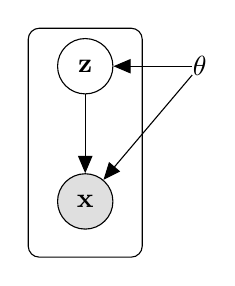
\begin{tikzpicture}[scale=1, transform shape]
                    \node[obs] (x1) {$\mathbf{x}$};
                    \node[latent, above=of x1] (z1) {$\mathbf{z}$};
                    \node[const, right=of z1] (theta1) {$\mathbf{\theta}$};
                    \edge {theta1} {z1};
                    \edge {theta1} {x1};
                    \edge {z1} {x1};
                    \plate [xscale=1.5] {} {(x1)(z1)} {} ;
                \end{tikzpicture}
            \end{center}
        }
        \item{
            $z \sim \pT(\bz)$
        }
        \item{
            Given $z$, $x \sim \pT(\bx \mid z)$
        }
        \item{
            We only observe $x \sim \pT(\bx)$
        }
        \item{
            $\pT(\bx) = \int_{z} \pT(\bx|\bz) \pT(\bz) d\bz$.
        }
    \end{itemize}

\end{frame}

% TODO(abora) : Don't have time now
% \begin{frame}{Latent Variable Models}{Example}
% \end{frame}

% \section{Problem Setting}

% \begin{frame}{Problem setting}
%     \begin{columns}[T]
%         \begin{column}{.7\textwidth}
%             \begin{itemize}
%                 \item{
%                     Parametric families of distributions $\pT(\bz)$ and $\pT(\bx \mid \bz)$.
%                 }
%                 \item{
%                     Assuption: There exists a $\theta^*$ such that data is generated by prior $p_{\theta^*}(\bz)$ and likelihood $p_{\theta^*}(\bx \mid \bz)$.
%                 }
%                 \item{
%                     Data generation process (image on the right)
%                 }
%                 \item{
%                     Dataset $\bX = \{\bx^{(i)}\}_{i=1}^N$  consisting of $N$ i.i.d. samples from this process
%                 }
%             \end{itemize}
%         \end{column}

%         \begin{column}{.2\textwidth}
%             \begin{tikzpicture}[scale=1, transform shape]
%                 \node[obs] (x1) {$\mathbf{x}$};
%                 \node[latent, above=of x1] (z1) {$\mathbf{z}$};
%                 \node[const, right=of z1] (theta1) {$\mathbf{\theta^*}$};
%                 \edge {theta1} {z1};
%                 \edge {theta1} {x1};
%                 \edge {z1} {x1};
%                 \plate [xscale=1.5] {} {(x1)(z1)} {$N$} ;
%             \end{tikzpicture}
%         \end{column}
%     \end{columns}
% \end{frame}

\section{Tasks}

% \begin{frame}{But what do we want?}
%     \pause
%     \begin{figure}
%         \centering
%         \includegraphics[width=0.8\textwidth]{steve_jobs}
%         \label{fig:steve_jobs}
%     \end{figure}
%     Image taken from Google Images
% \end{frame}

\begin{frame}{Tasks}
    \begin{columns}[T]
        \begin{column}{.7\textwidth}
            \begin{itemize}
                \item ML/MAP inference on $\theta$. \\
                \qquad mimic data generation
                \item Posterior inference on $z$ given $x$. \\
                \qquad coding/data representation.
                \item Marginal inference on $x$ \\
                \qquad denoising, inpainting, super-resolution.
            \end{itemize}
            Want efficient algorithms for all, with minimal assumptions.
        \end{column}

        \begin{column}{.2\textwidth}
            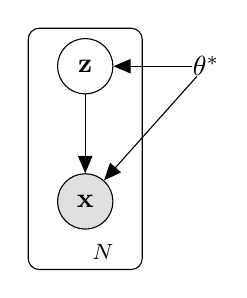
\begin{tikzpicture}[scale=1, transform shape]
                \node[obs] (x1) {$\mathbf{x}$};
                \node[latent, above=of x1] (z1) {$\mathbf{z}$};
                \node[const, right=of z1] (theta1) {$\mathbf{\theta^*}$};
                \edge {theta1} {z1};
                \edge {theta1} {x1};
                \edge {z1} {x1};
                \plate [xscale=1.5] {} {(x1)(z1)} {$N$} ;
            \end{tikzpicture}
        \end{column}
    \end{columns}
\end{frame}

\begin{frame}{Why is this hard?}
    \begin{columns}[T]
        \begin{column}{.5\textwidth}
            \begin{itemize}
                \item{
                    Lots of stuff hidden from us, we only see $x$.
                }
                \item {
                    Data generation process can be complicated
                }
            \end{itemize}
        \end{column}

        \begin{column}{.4\textwidth}
            \begin{figure}
                \centering
                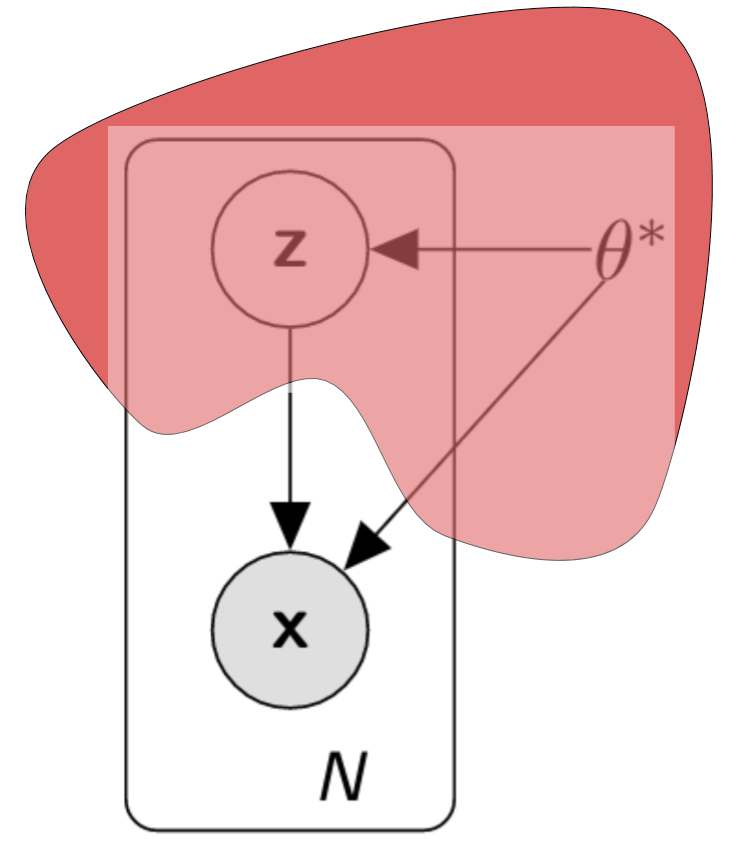
\includegraphics[width=\textwidth]{latent_hidden}
            \end{figure}

        \end{column}
    \end{columns}
\end{frame}

\begin{frame}{Ideas?}
    \begin{figure}
        \centering
        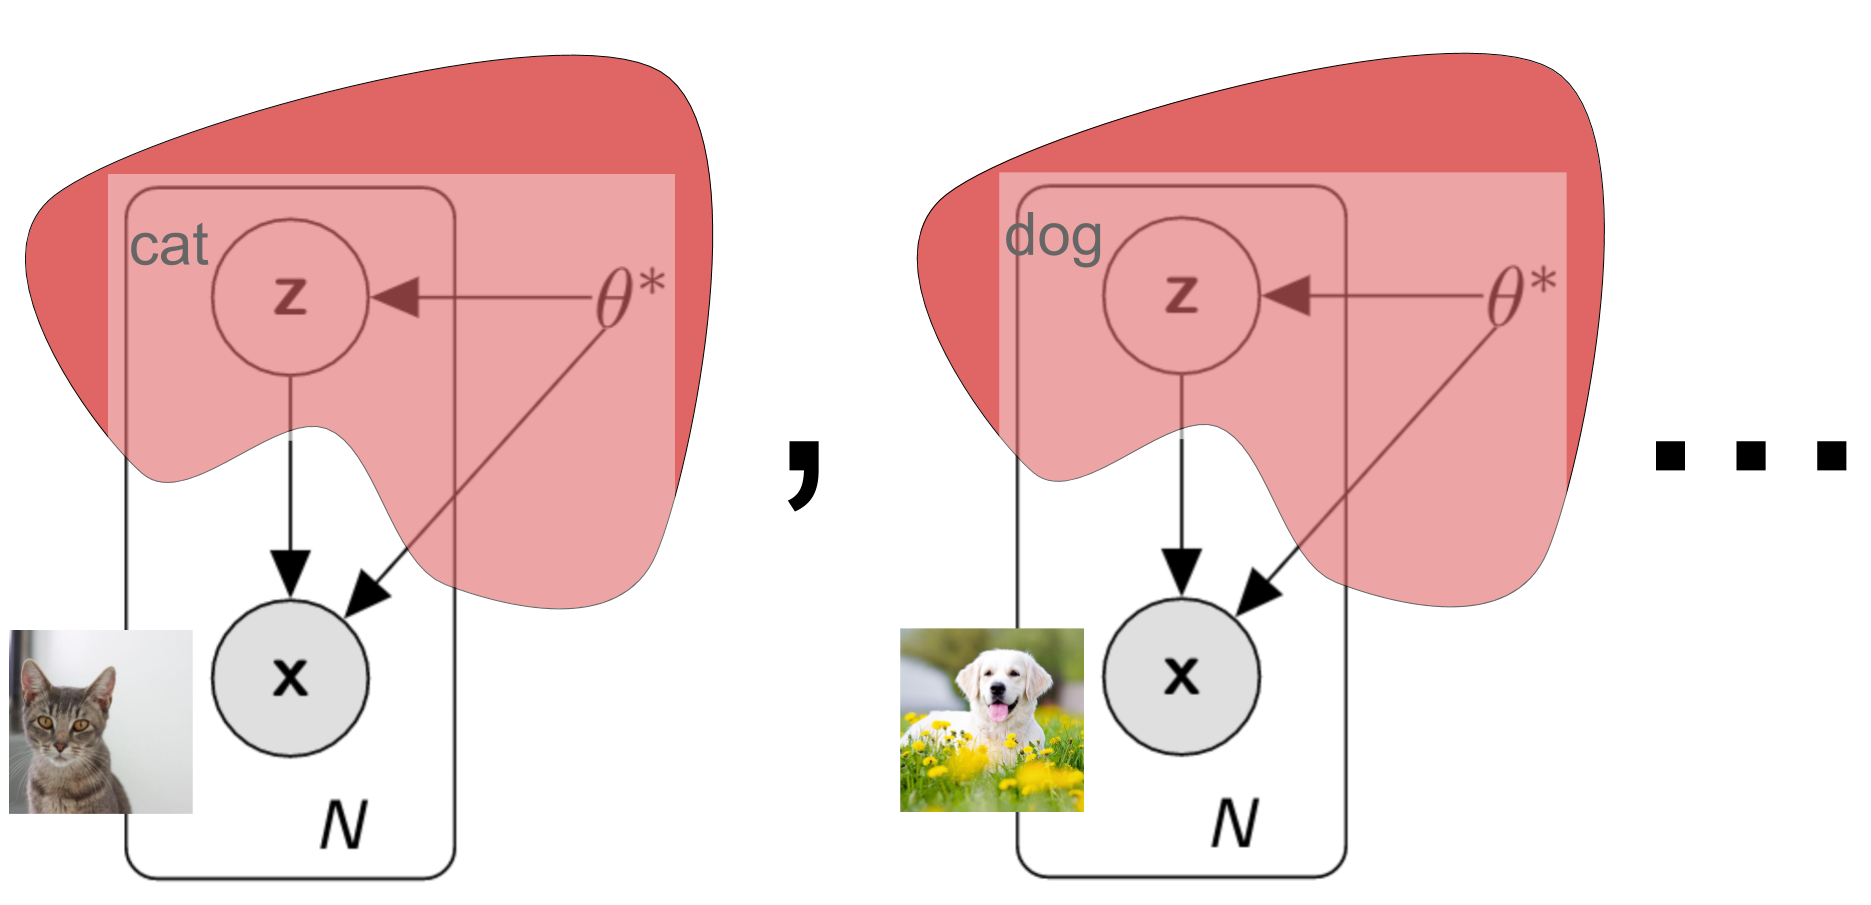
\includegraphics[width=0.8\textwidth]{latent_hidden_concrete}
    \end{figure}
    Given only images, we want
    \begin{itemize}
        \item $\theta$ close to $\theta^*$
        \item An approximation to $p_{\theta^*}(z \mid x)$
        \item A good model of $p_{\theta^*}(x)$
    \end{itemize}
    {\small Images from Google Images}
\end{frame}

\section{Known Approaches}

\begin{frame}{Some approaches}{Idea 1}

    \begin{itemize}
        \item {
            Integrate out $z$. Maximize marginal likelihood $$\pT(\bx) = \int_{z} \pT(x \mid z) \pT(z) dz$$ . \\
            \pause
            Problem : nasty integral
        }
    \end{itemize}

    \begin{figure}
        \centering
        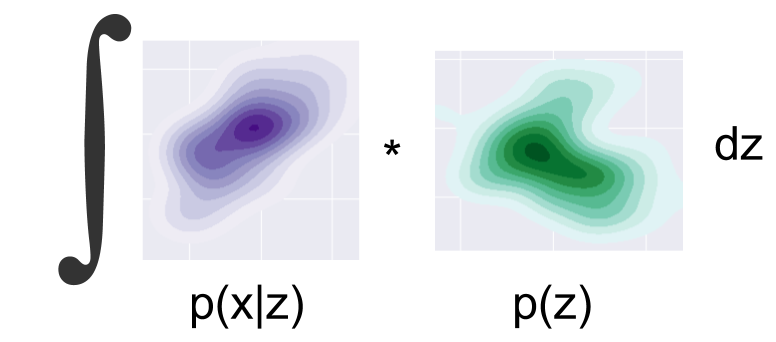
\includegraphics[width=0.6\textwidth]{marginal_likelihood_illustration}
    \end{figure}
\end{frame}


\begin{frame}{Some approaches}{Idea 2}
    \begin{itemize}
        \item {
            Alternating optimization between $z$ and $\theta$ : Expectation Maximization.

            \vspace{3mm}
            Example : kMeans
            \begin{itemize}
                \item $\theta$ contains cluster centres.
                \item for every $x_i$, $z_i$ is the cluster id.
            \end{itemize}
        }
        \begin{figure}
            \centering
            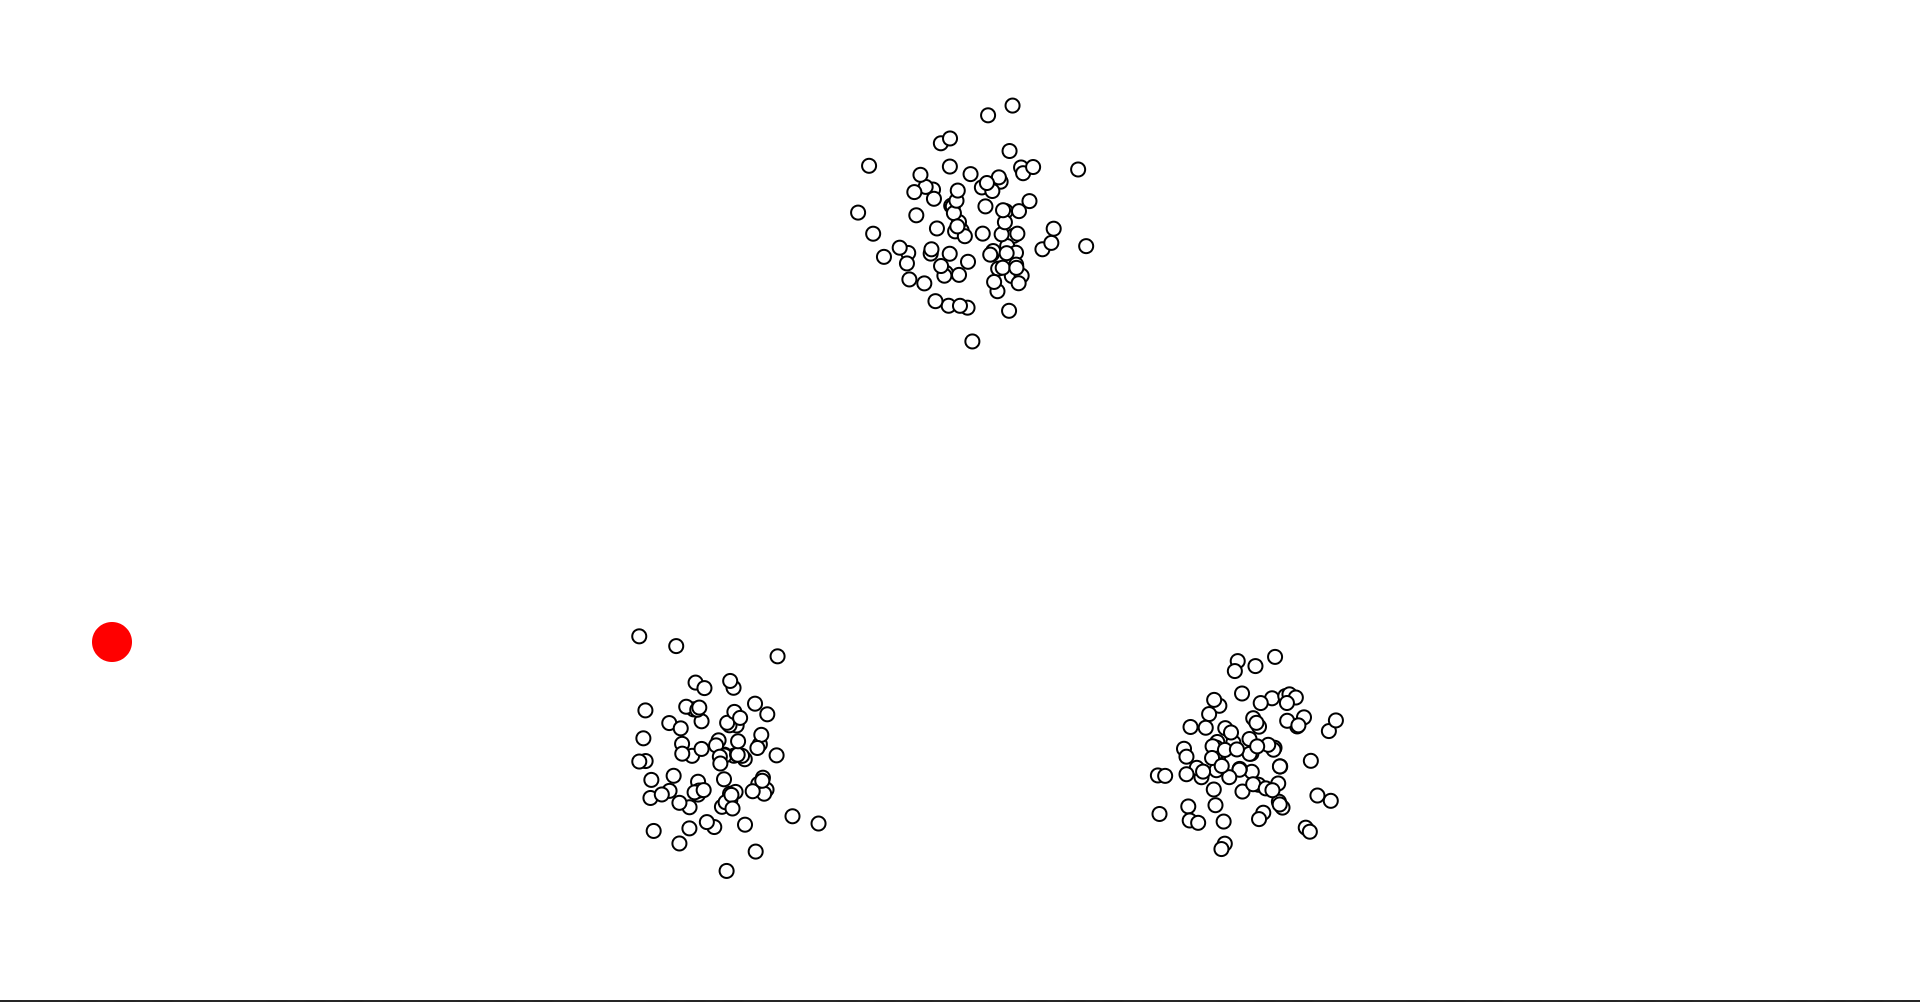
\includegraphics[width=0.7\textwidth]{kmeans1}
        \end{figure}
    \end{itemize}
    {\small Image from https://www.naftaliharris.com/blog/visualizing-k-means-clustering/}
\end{frame}

\begin{frame}{Some approaches}{Idea 2}
    \begin{itemize}
        \item {
            Alternating optimization between $z$ and $\theta$ : Expectation Maximization.

            \vspace{3mm}
            Example : kMeans
            \begin{itemize}
                \item $\theta$ contains cluster centres.
                \item for every $x_i$, $z_i$ is the cluster id.
            \end{itemize}
        }
        \begin{figure}
            \centering
            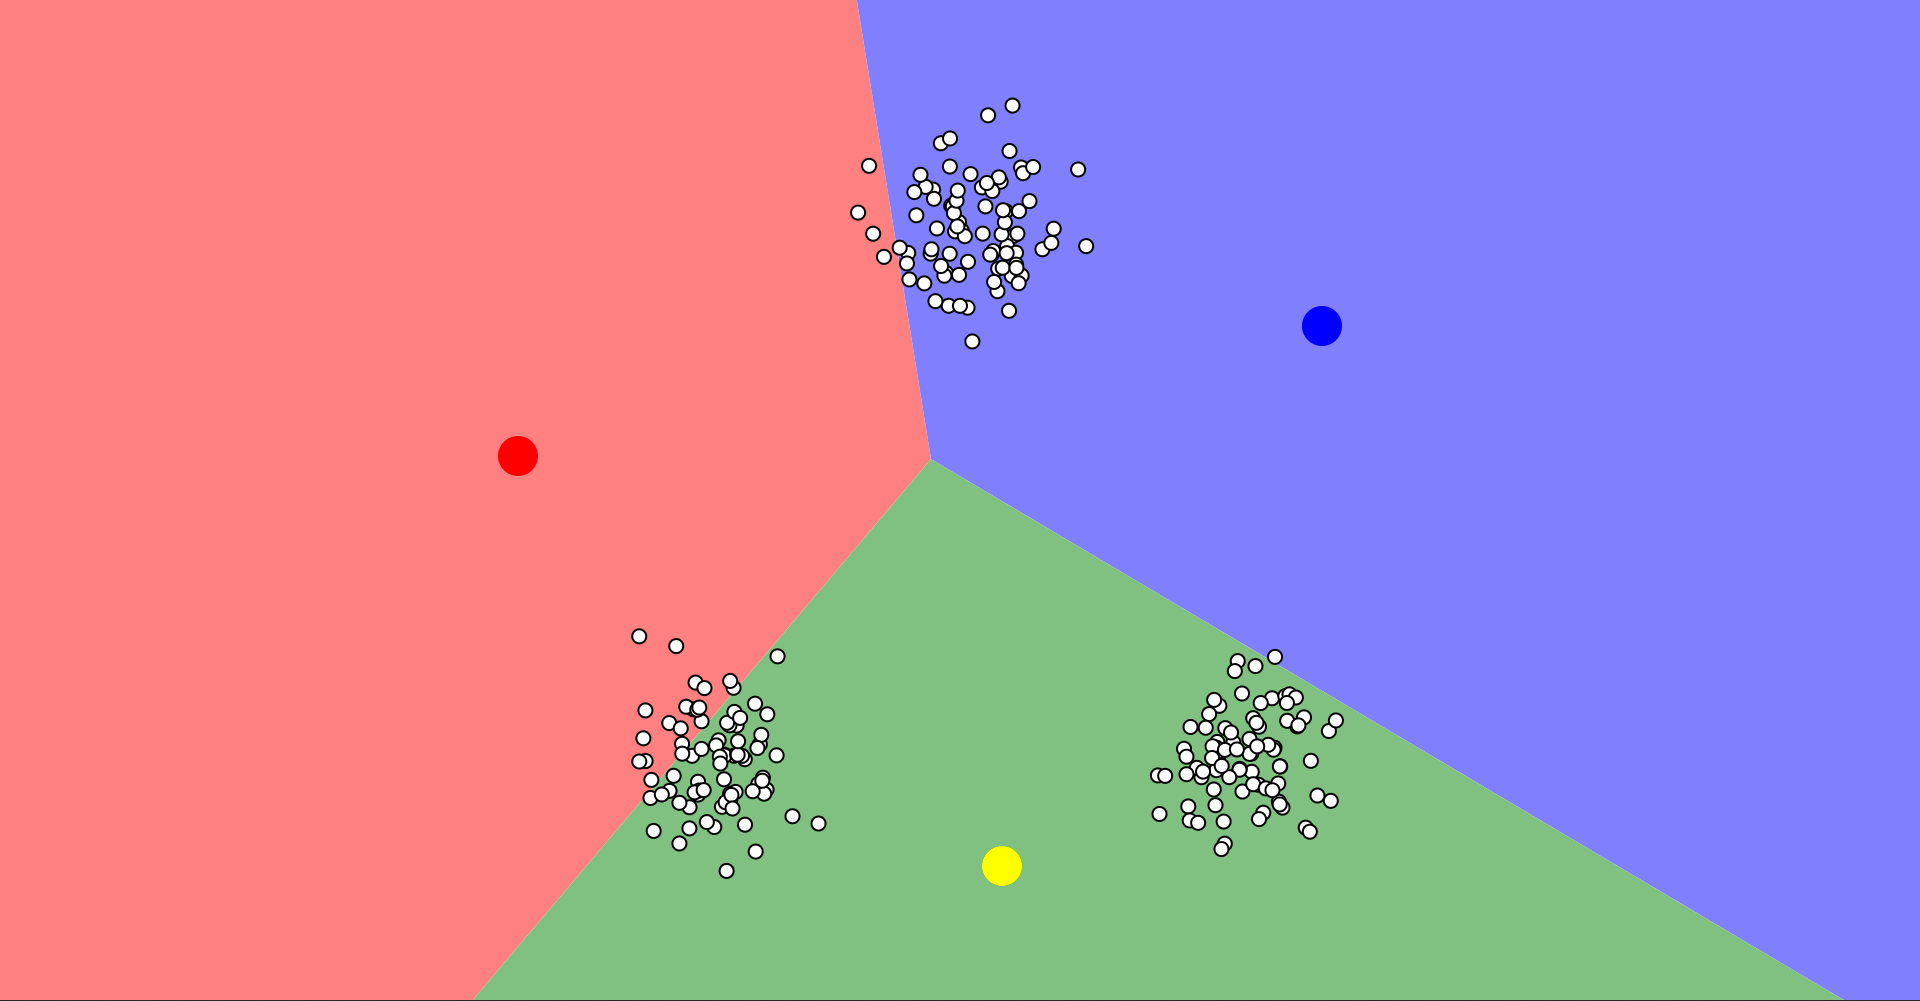
\includegraphics[width=0.7\textwidth]{kmeans2}
        \end{figure}
    \end{itemize}
    {\small Image from https://www.naftaliharris.com/blog/visualizing-k-means-clustering/}
\end{frame}
\begin{frame}{Some approaches}{Idea 2}
    \begin{itemize}
        \item {
            Alternating optimization between $z$ and $\theta$ : Expectation Maximization.

            \vspace{3mm}
            Example : kMeans
            \begin{itemize}
                \item $\theta$ contains cluster centres.
                \item for every $x_i$, $z_i$ is the cluster id.
            \end{itemize}
        }
        \begin{figure}
            \centering
            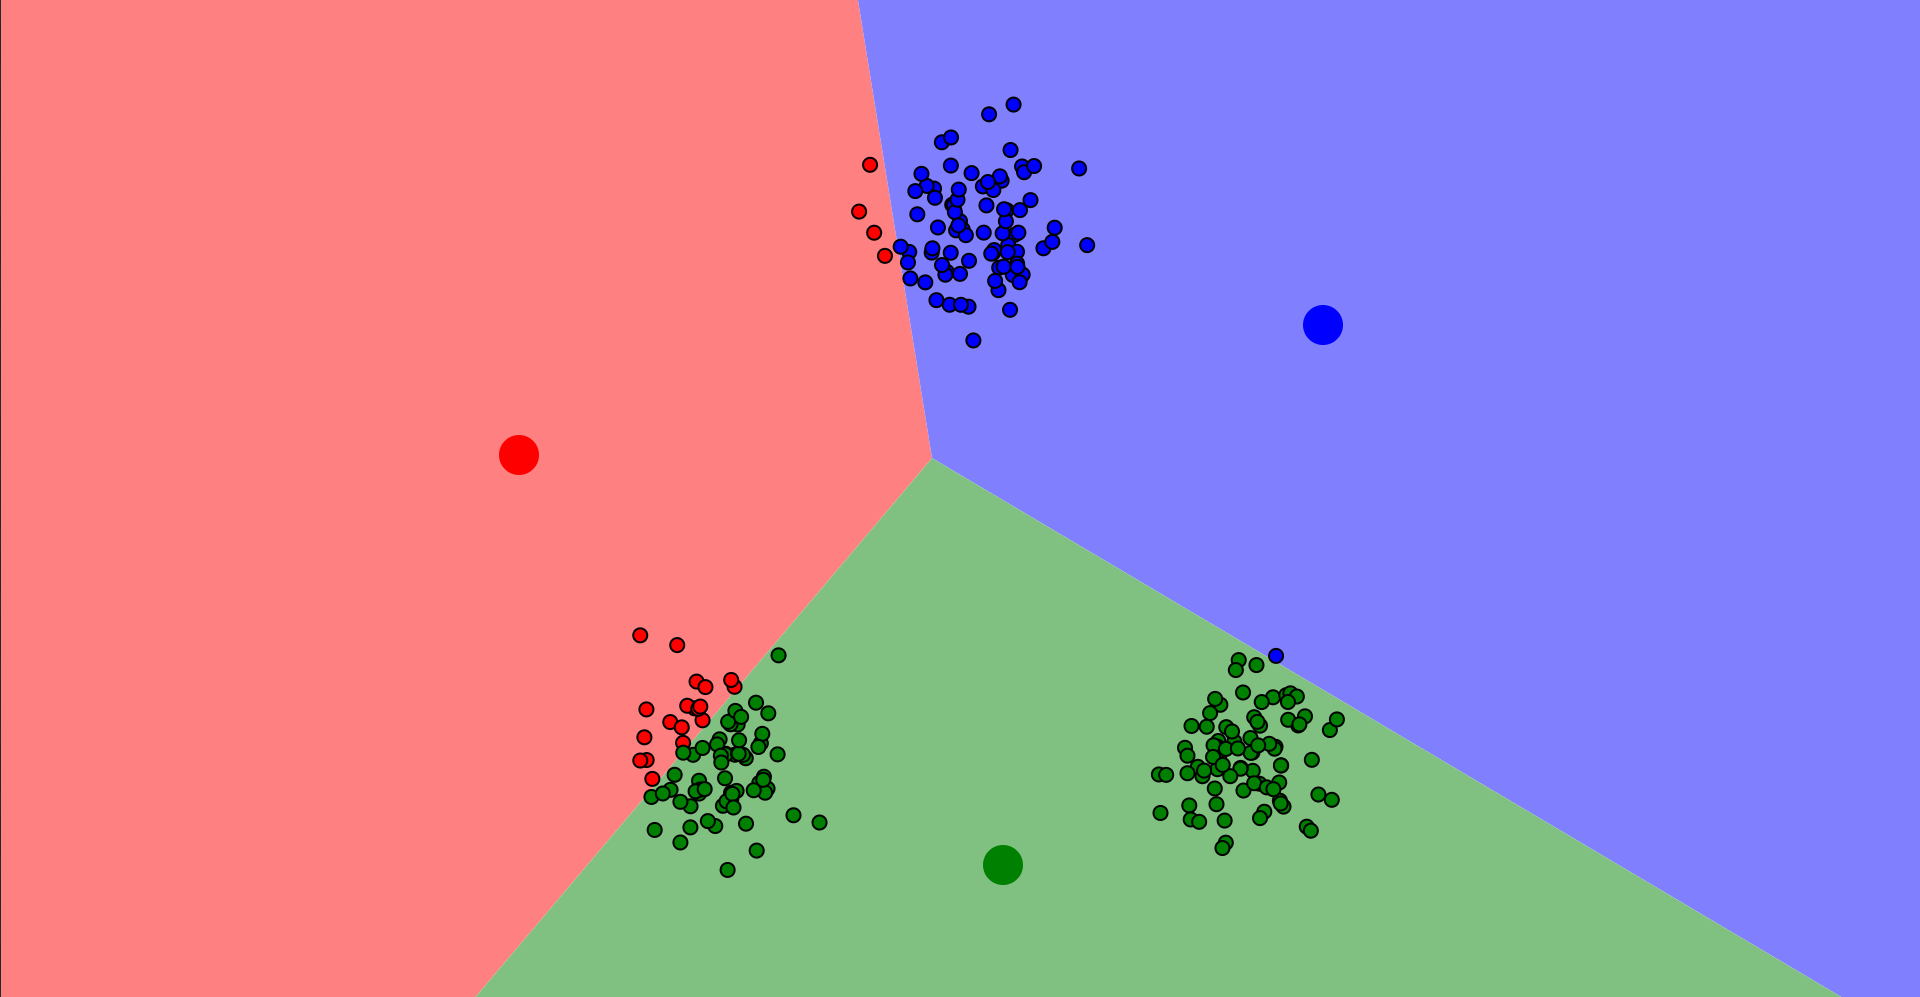
\includegraphics[width=0.7\textwidth]{kmeans3}
        \end{figure}
    \end{itemize}
    {\small Image from https://www.naftaliharris.com/blog/visualizing-k-means-clustering/}
\end{frame}
\begin{frame}{Some approaches}{Idea 2}
    \begin{itemize}
        \item {
            Alternating optimization between $z$ and $\theta$ : Expectation Maximization.

            \vspace{3mm}
            Example : kMeans
            \begin{itemize}
                \item $\theta$ contains cluster centres.
                \item for every $x_i$, $z_i$ is the cluster id.
            \end{itemize}
        }
        \begin{figure}
            \centering
            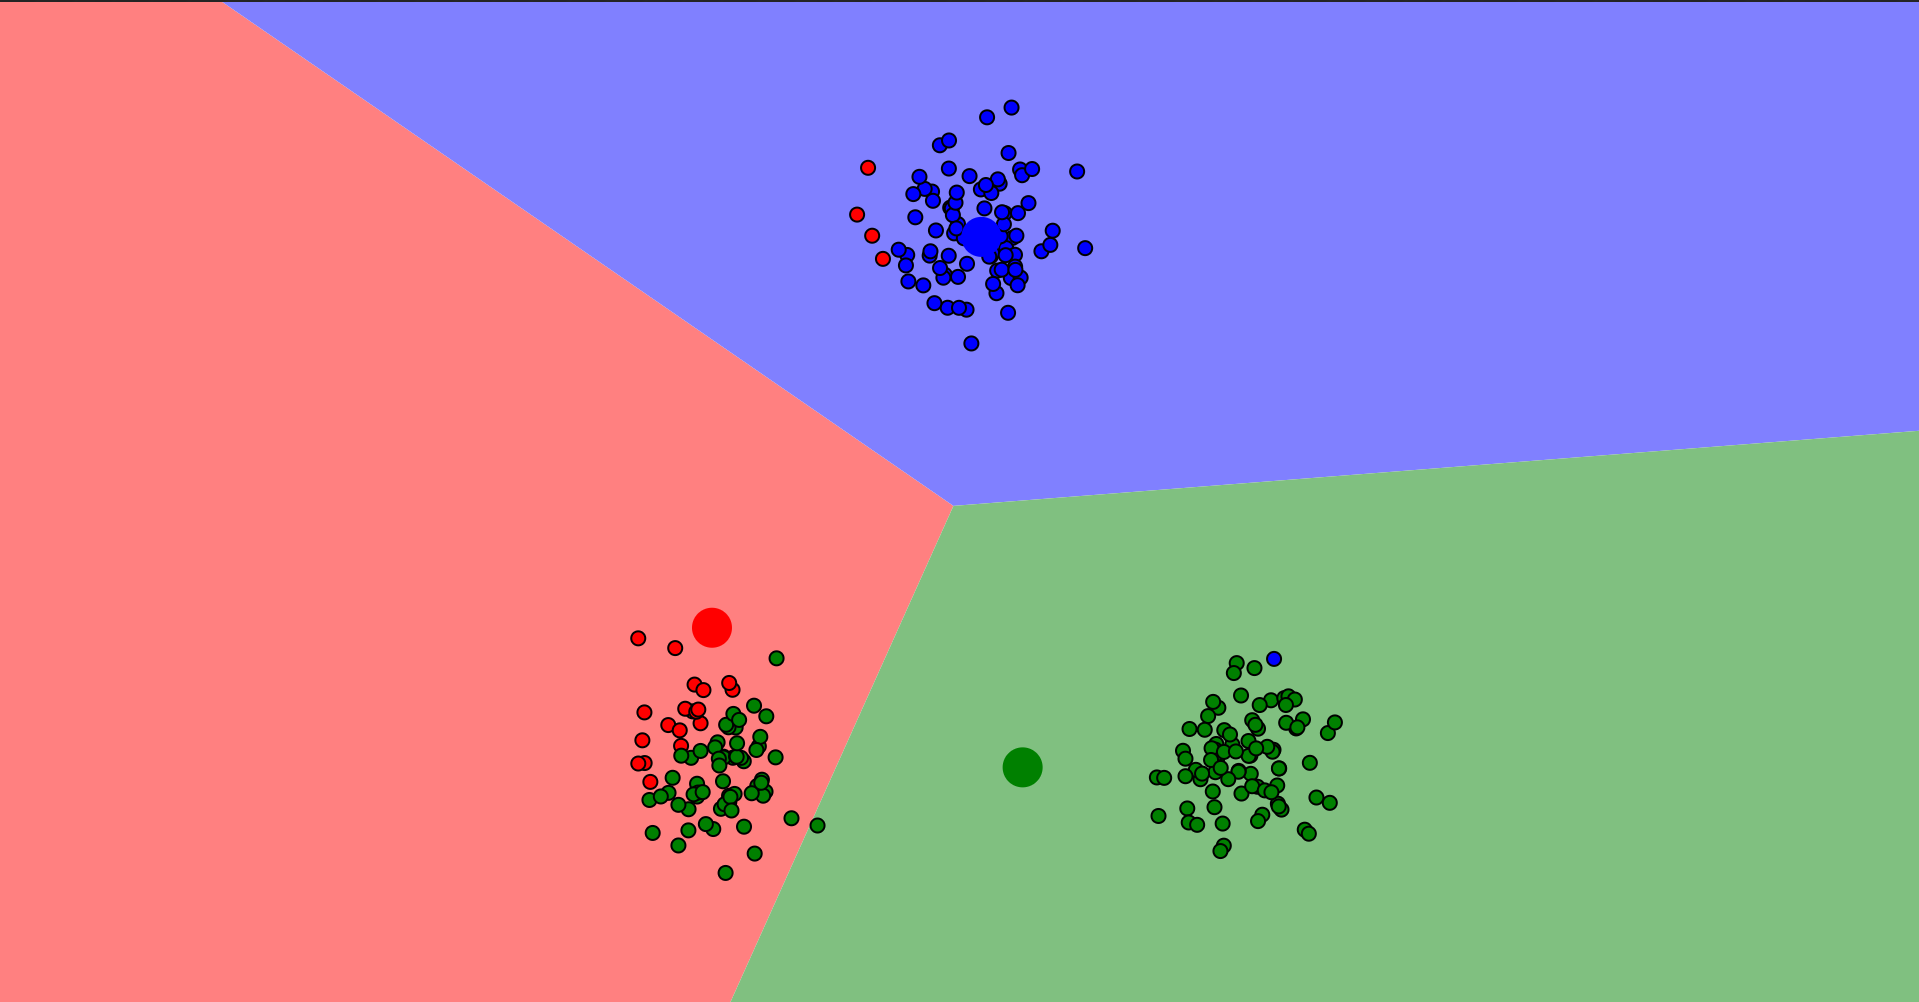
\includegraphics[width=0.7\textwidth]{kmeans4}
        \end{figure}
    \end{itemize}
    {\small Image from https://www.naftaliharris.com/blog/visualizing-k-means-clustering/}
\end{frame}
\begin{frame}{Some approaches}{Idea 2}
    \begin{itemize}
        \item {
            Alternating optimization between $z$ and $\theta$ : Expectation Maximization.

            \vspace{3mm}
            Example : kMeans
            \begin{itemize}
                \item $\theta$ contains cluster centres.
                \item for every $x_i$, $z_i$ is the cluster id.
            \end{itemize}
        }
        \begin{figure}
            \centering
            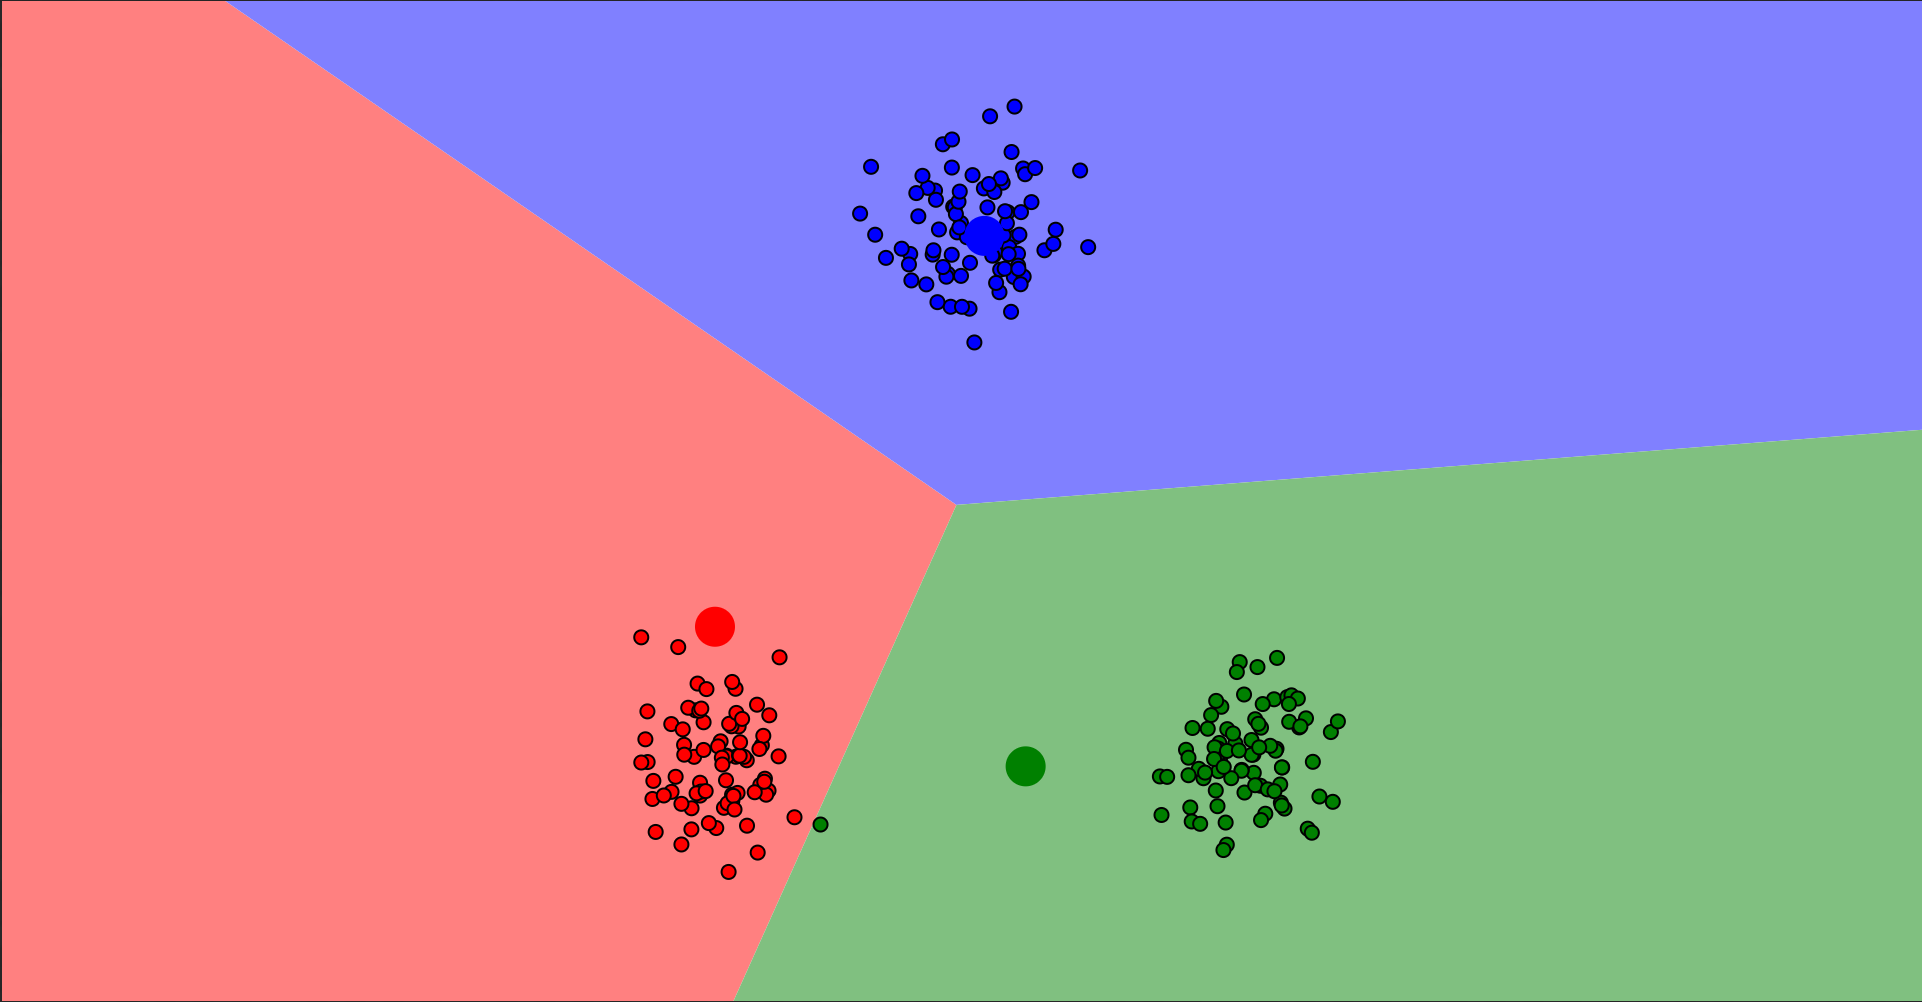
\includegraphics[width=0.7\textwidth]{kmeans5}
        \end{figure}
    \end{itemize}
    {\small Image from https://www.naftaliharris.com/blog/visualizing-k-means-clustering/}
\end{frame}
\begin{frame}{Some approaches}{Idea 2}
    \begin{itemize}
        \item {
            Alternating optimization between $z$ and $\theta$ : Expectation Maximization.

            \vspace{3mm}
            Example : kMeans
            \begin{itemize}
                \item $\theta$ contains cluster centres.
                \item for every $x_i$, $z_i$ is the cluster id.
            \end{itemize}
        }
        \begin{figure}
            \centering
            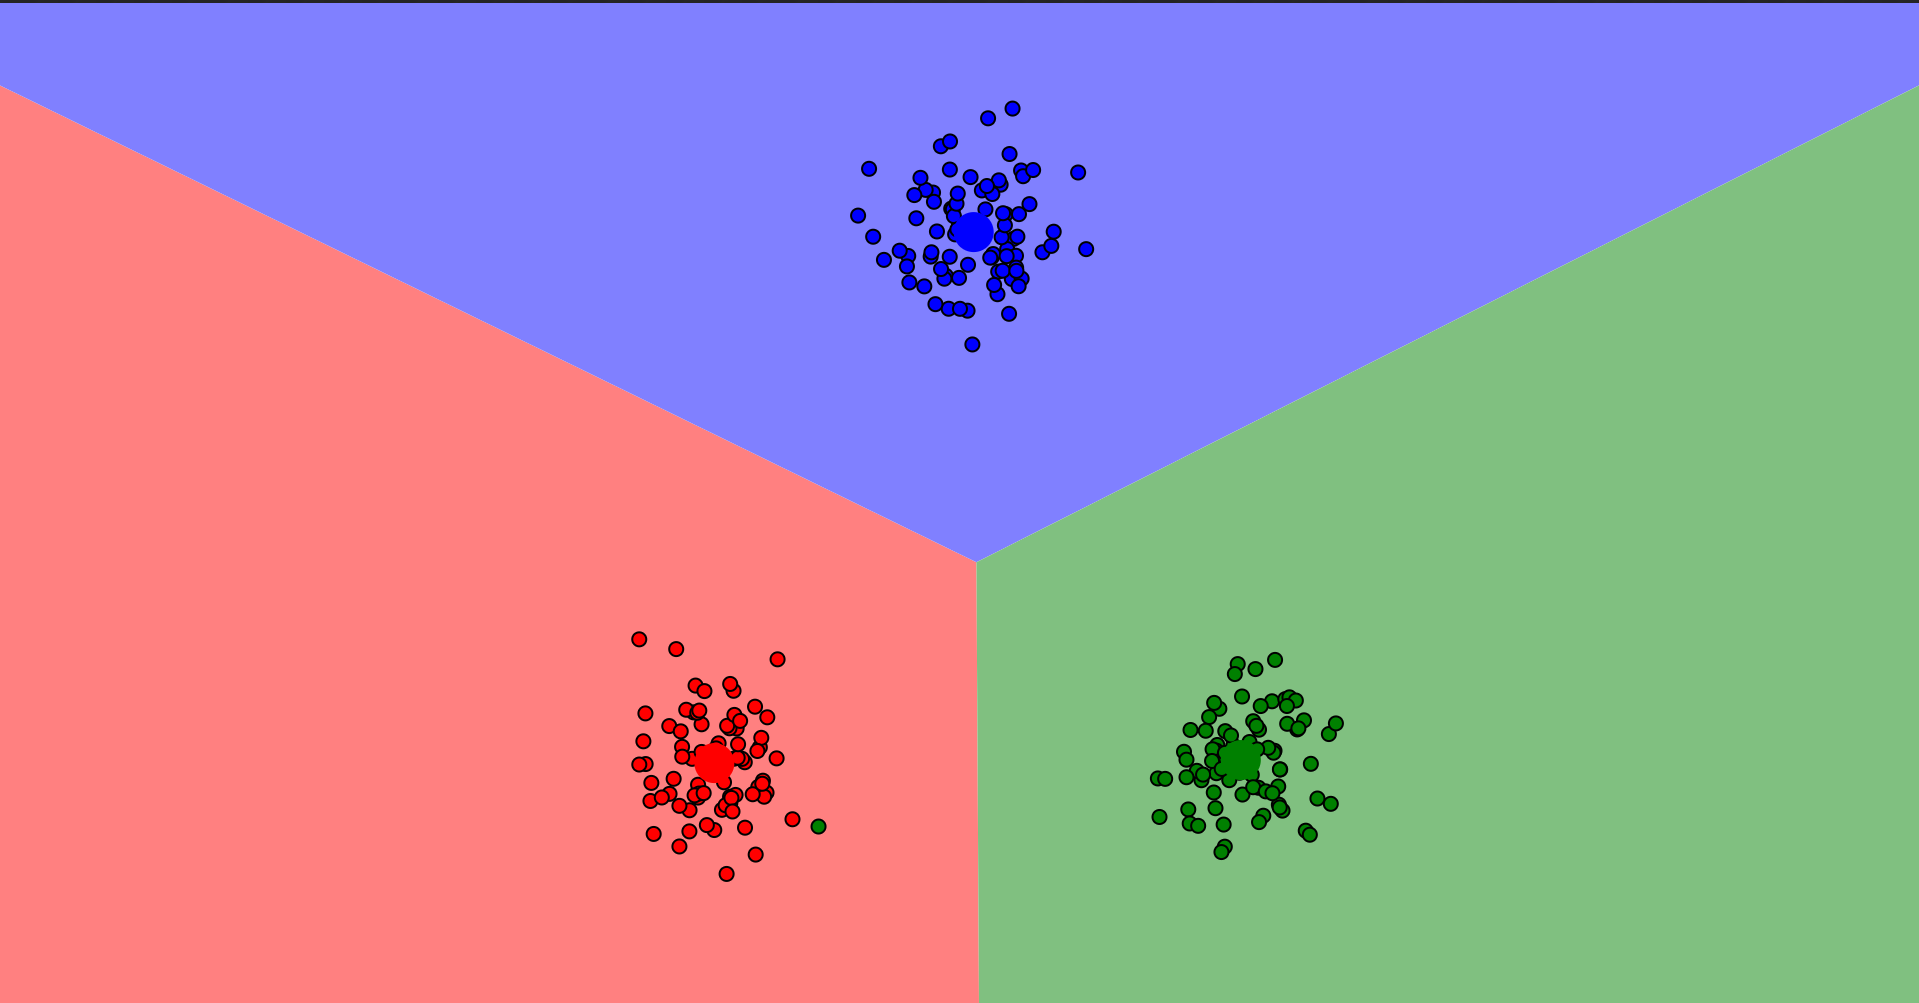
\includegraphics[width=0.7\textwidth]{kmeans6}
        \end{figure}
    \end{itemize}
    {\small Image from https://www.naftaliharris.com/blog/visualizing-k-means-clustering/}
\end{frame}

\begin{frame}{Some approaches}{Idea 2}
    \begin{itemize}
        \item {
            Alternating optimization between $z$ and $\theta$ : Expectation Maximization.
        }

        \vspace{3mm}
        Problem : Posterior $\pT(\bz \mid \bx)$ may not be tractable.
    \end{itemize}
\end{frame}


% \begin{frame}{Known algorithms}

% Most use some kind of simplifying assumption.

% Examples:
%     \begin{itemize}
%         \item {
%             Marginal likelihood, $\pT(\bx)$, is tractable : Maximize marginal likelihood. \\
%             \vspace{5mm}
%             \pause {\color{red} Q : What is tractable?} \\
%             \pause {A : Either closed form is known or the value can be easily computed numerically}
%         }
%     \end{itemize}
% \end{frame}

% \begin{frame}{Known algorithms}

% Most use some kind of simplifying assumption. Examples:
%     \begin{itemize}
%         \item {
%             Marginal likelihood, $\pT(\bx)$, is tractable : Maximize marginal likelihood.
%         }
%         \item{
%             Posterior, $\pT(\bz \mid \bx)$ is tractable : Expectation Maximization
%         }
%         \item{
%             Mean Field integrals are tractable: Mean Field Variational approximation. Assume posterior factorizes over subsets. Closed form integrals for optimal posterior available (using calculus of variations, and thus the name)
%         }
%         \item{
%             Dataset is small : Monte Carlo Expectation Maximization.
%         }
%     \end{itemize}

%     \vspace{5mm}
%     None of this is assumed in this paper.
% \end{frame}

\section{Variational Inference}

\begin{frame}{Enter Variational Inference!}
    \begin{columns}[T]
        \begin{column}{.7\textwidth}
            \begin{itemize}
                \item {
                    Problem: We want to estimate some distribution $\pT(\cdot)$, but direct estimation is hard.
                }
            \end{itemize}
        \end{column}
        \begin{column}{.3\textwidth}
            \begin{figure}
                \centering
                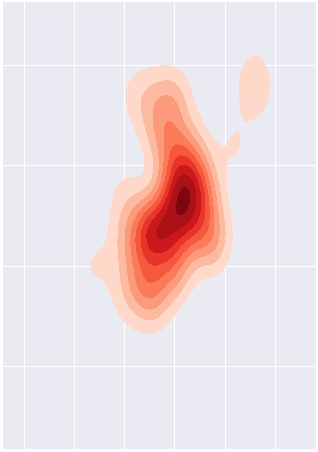
\includegraphics[width=\textwidth]{dist1}
            \end{figure}
        \end{column}
    \end{columns}
\end{frame}

\begin{frame}{Enter Variational Inference!}
    \begin{columns}[T]
        \begin{column}{.7\textwidth}
            \begin{itemize}
                \item {
                    Problem: We want to estimate some distribution $\pT(\cdot)$, but direct estimation is hard.
                }
                \item{
                    Solution
                    \begin{itemize}
                        \item {
                            Approximate $\pT(\cdot)$ with a simpler distribution $\qPhi(\cdot)$.
                        }
                        \item {
                            Find parameters $\phi$ such that the approximation is ``close".
                        }
                    \end{itemize}
                }
            \end{itemize}
        \end{column}
        \begin{column}{.3\textwidth}
            \begin{figure}
                \centering
                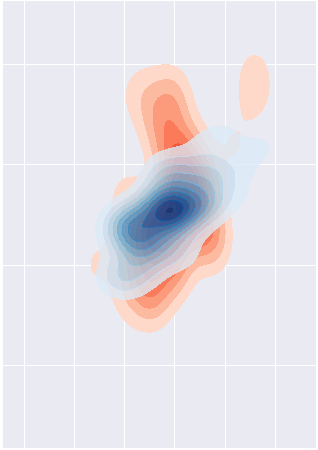
\includegraphics[width=\textwidth]{dist2}
            \end{figure}
        \end{column}
    \end{columns}
\end{frame}

\begin{frame}{Variational Inference -- our setting}
    \begin{columns}[T]
        \begin{column}{.7\textwidth}
            \begin{itemize}
                \item Since the posterior $\pT(\bz \mid \bx)$ is intractable, use variational approximation $\qPhi(\bz \mid \bx)$.
                \item $\qPhi(\bz \mid \bx)$ : probabilistic {\color{red} encoder}
                \item $\pT(\bx \mid \bz)$ : probabilistic {\color{blue} decoder}
            \end{itemize}
        \end{column}
        \begin{column}{.3\textwidth}
            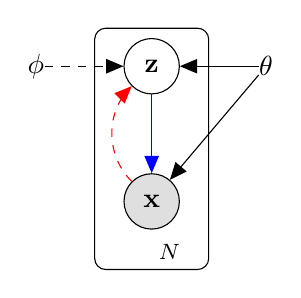
\begin{tikzpicture}[scale=1, transform shape]
                \node[obs] (x1) {$\mathbf{x}$};
                \node[latent, above=of x1] (z1) {$\mathbf{z}$};
                \node[const, left=of z1] (phi1) {$\mathbf{\phi}$};
                \node[const, right=of z1] (theta1) {$\mathbf{\theta}$};
                \edge [dashed] {phi1} {z1};
                \edge {theta1} {z1};
                \edge {theta1} {x1};
                \draw (x1) edge[out=135,in=225,->,dashed, color=red] (z1);
                %\draw (z1) edge[out=315,in=45,->] (x1);
                \edge[color=blue] {z1} {x1};
                \plate [xscale=1.5] {} {(x1)(z1)} {$N$} ;
            \end{tikzpicture}
        \end{column}
    \end{columns}
\end{frame}

% \section{Variational Lower Bound}

% \begin{frame}{Variational Lower Bound}
%     \begin{itemize}
%         \item{
%             We can write marginal likelihood as an expectation over the posterior
%             % \pT(\bxi) &=  \frac{\pT(\bxi,\bz)}{\pT(\bz \mid \bxi)} \\
%             $$\log \pT(\bxi) = \Exp{\pT(\bz|\bxi)}{- \log \pT(\bz|\bxi) + \log \pT(\bxi,\bz)}$$
%         }
%         \item{
%             Lets replace intractable posterior $\pT(\bz \mid \bxi)$ by its tractable approximation $\qPhi(\bz \mid \bxi)$.
%             $$\LB{}{\bxi} = \Exp{\qPhi(\bz|\bxi)}{- \log \qPhi(\bz|\bxi) + \log \pT(\bxi,\bz)}$$
%         }

%         \item {
%             \pause {\color{red} Q : Will the approximate likelihood be larger or smaller?} \\
%             \pause {Hint : Higher likelihood is better} \\
%             \pause {A : Approximation models the data less well and hence approximate likelihood should be smaller}
%         }
%     \end{itemize}
% \end{frame}


\begin{frame}{Variational Lower Bound}
    \begin{itemize}
        \item{
            Using approximation leads to smaller marginal likelihood.
        }
        \item{
        Lower bound on marginal likehood in terms of the variational approximation:
            % $$\LB{}{\bxi} = \Exp{\qPhi(\bz|\bxi)}{- \log \qPhi(\bz|\bxi) + \log \pT(\bxi,\bz)}$$
        }

        \begin{figure}
            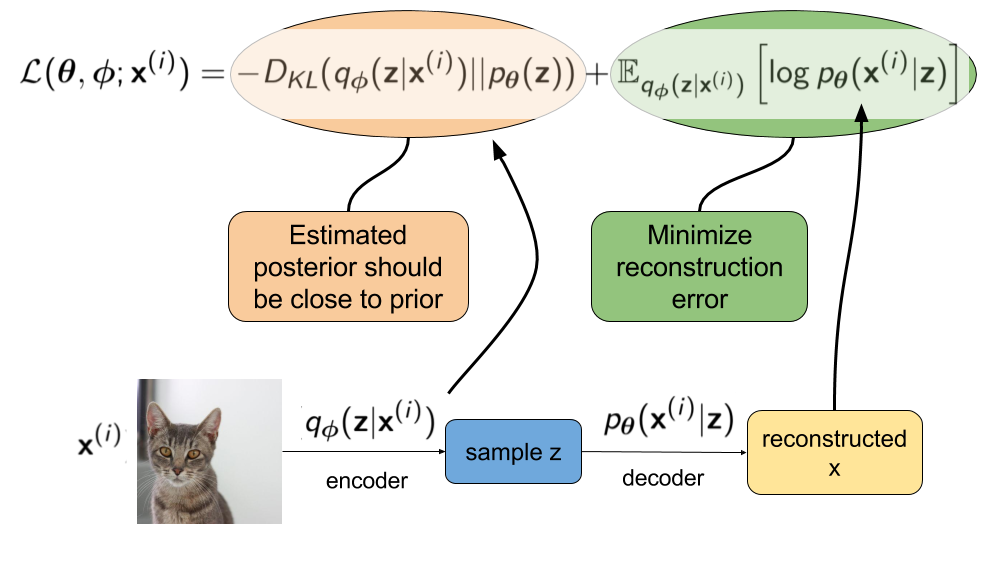
\includegraphics[width=0.9\textwidth]{lower_bound2}
        \end{figure}

        \item{
            Lower bound is tractable. So, we maximize it with respect to $\theta$ and $\phi$ jointly.
        }
    \end{itemize}

\end{frame}


% \begin{frame}{Variational Lower Bound}
%     \begin{itemize}
%         \item {
%             Lower Bound proof
%             \begin{itemize}
%                 \item {
%                     We can write $$\log \pT(\bxi) = D_{KL}(\qPhi(\bz|\bxi)||\pT(\bz|\bxi)) + \LB{}{\bxi}$$. Since KL divergence is non-negative, we have that $$\log \pT(\bxi) \geq \LB{}{\bxi}$$.
%                 }
%                 \item {
%                     Notice that the bound is tight
%                 }
%             \end{itemize}
%         }
%         \item{
%             Observation : KL term is intractable. Lower bound is tractable
%         }
%         \item {
%             Idea: Ignore KL term, maximize lower bound with respect to $\theta$ and $\phi$.
%         }
%     \end{itemize}
% \end{frame}

\section{Parametrization of distributions}

\begin{frame}{Where is Deep Learning?}

    \begin{figure}
        \centering
        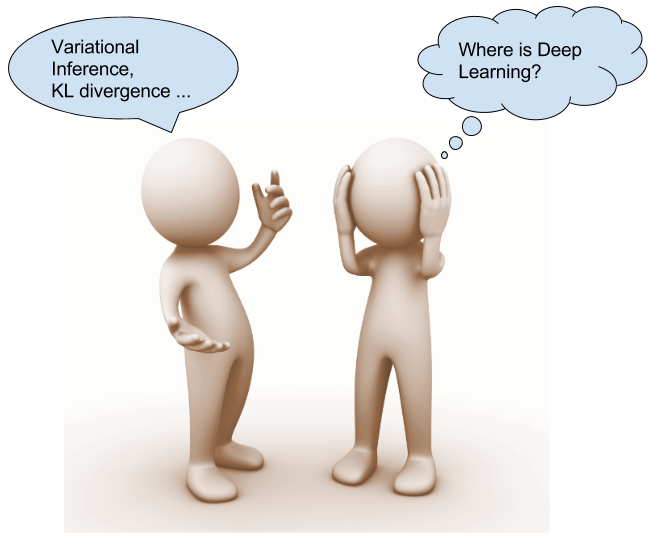
\includegraphics[width=0.7\textwidth]{where_is_deep_learning}
        \label{fig:where_is_deep_learning}
    \end{figure}
    {\small Image taken Google Images (modified)}
\end{frame}

\begin{frame}{Parametrizing distributions}

    {\color{red} Ideas?}
    \begin{itemize}
        \item {
            \pause
            Since we did not assume tractable posteriors, can use any artibrary functions for generative and variational part.
        }
        \item {
            Only requirement - we should be able to optimize wrt $\theta$ and $\phi$.
        }
        \item {
            For gradient based algorithms, we want a paramteric family which is differentiable wrt inputs and parameters.
        }
        \item{
            Can use neural networks.
            \pause
            \begin{figure}
                \centering
                
\includegraphics[width=0.3\textwidth]{finally}
            \end{figure}
        }
        {\small Image from Google Images}
      \end{itemize}
\end{frame}


\begin{frame}{Example : Variational Autoencoder}
    \begin{columns}[T]
        \begin{column}{.5\textwidth}
            \begin{itemize}
                \item {
                    $\pT(\bz) = \mathcal{N}(\bz; \bzero, \bI)$
                }
                \item {
                    $\pT(\bx|\bz)$ be a "simple" distribution whose distribution parameters are computed from $\bz$ with a neural network.
                }
                \item {
                    Assume $\qPhi(\bz|\bxi) = \mathcal{N}(\bz; \bmu^{(i)}, \bsigma^{2 (i)} \bI)$, where $\mu$, and $\sigma$ are predicted using a neural network
                }
            \end{itemize}
        \end{column}
        \begin{column}{0.5\textwidth}
            \begin{figure}
                \centering
                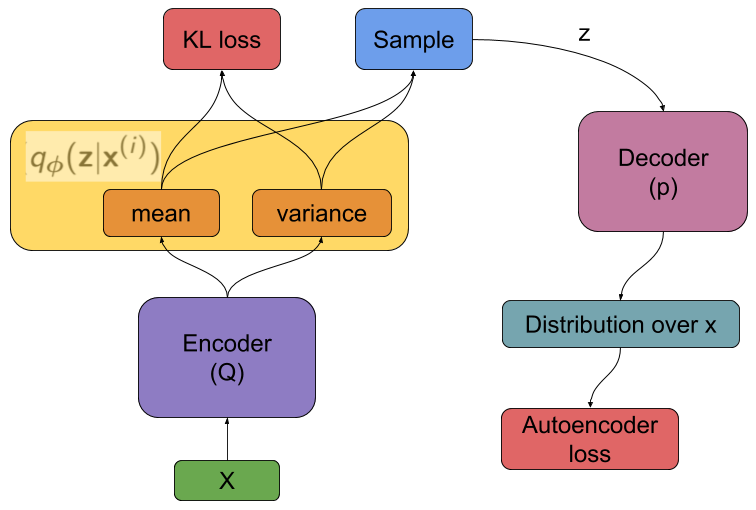
\includegraphics[width=\textwidth]{vae_no_param}
            \end{figure}
        \end{column}
    \end{columns}
\end{frame}


\begin{frame}{Gradient based optimization : Na{\"i}ve method}
    \begin{itemize}
        \item{
            Lower bound is
            \begin{align*}
                \LB{}{\bxi} &= -D_{KL}(\qPhi(\bz|\bxi) || \pT(\bz)) + \Exp{\qPhi(\bz|\bxi)}{\log \pT(\bxi | \bz)} \\
                &= \Exp{\qPhi(\bz)}{f(\bz)}
            \end{align*}
        }
        \item {Monte Carlo estimator:
            \begin{align*}
                \nabla_{\bphi} \Exp{\qPhi(\bz)}{f(\bz)}
                &= \Exp{\qPhi(\bz)}{f(\bz) \nabla_{\qPhi(\bz)} \log \qPhi(\bz) } \\
                &\simeq \frac{1}{L} \sum_{l=1}^L f(\bzl) \nabla_{\qPhi(\bzl)} \log \qPhi(\bzl) \\
                 \text{\quad where \quad} \bzl &\sim \qPhi(\bz|\bxi)
            \end{align*}
        }
        \item {
            This has very high variance.
            \pause {\color{red} Q : Why?} \\
            \pause {A : Gradient of log of probability. Probability very close to zero means very large values.
            }
        }
    \end{itemize}

\end{frame}


\begin{frame}{The reparametrization trick}
    \begin{itemize}
        \item{
            Problem in na{\"i}ve method : learnable parameters responsible for producing probabilities.
        }
        \item{
            Observation: We don't need those probabilities, just an expectation taken using them.
        }
        \item{
            Solution
            \begin{itemize}
                \item {
                    Instead of producing probability for each $z$, produce $z$ directly
                }
                \item {
                    Make sure the distribution of $z$ is the same.
                }
                \item{
                    For randomness in $z$ generation, use a deterministic function with noise as input. i.e.
                    $$g_{\phi}(z, \epsilon) = \widetilde{z} \sim q_{\phi}(z|x), \ \epsilon \sim p(\epsilon)$$
                }
            \end{itemize}
        }
        \item {
            Now we can write expectations in terms of $p(\epsilon)$.
            \begin{align*}
                \Exp{\qPhi(\bz|\bxi)}{f(\bz)}
                &= \Exp{p(\beps)}{f(\gPhi(\beps,\bxi))} \simeq \frac{1}{L} \sum_{l=1}^L{f(\gPhi(\bepsl,\bxi))} \\
                \text{\quad where \quad} \bepsl &\sim p(\beps)
            \end{align*}
        }
    \end{itemize}
\end{frame}

\begin{frame}{Reparametrization for VAE}
    \begin{figure}
        \centering
        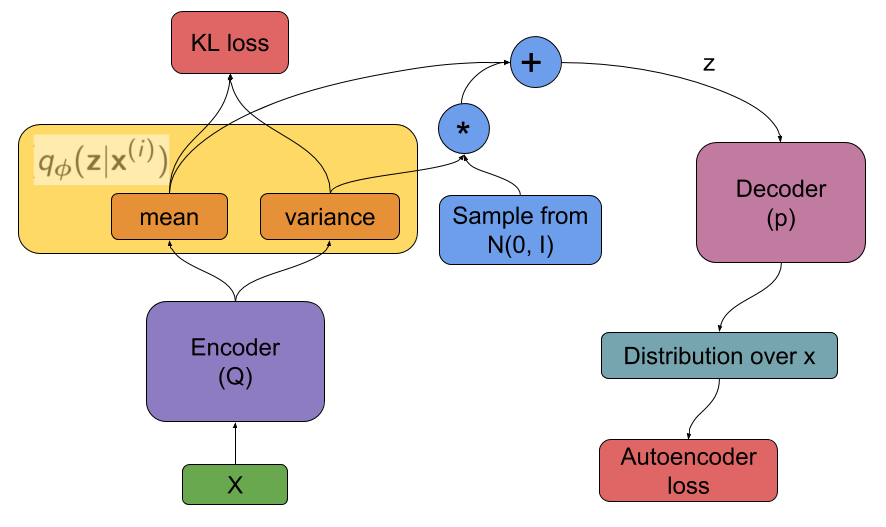
\includegraphics[width=\textwidth]{vae_param}
    \end{figure}
\end{frame}

\section{Putting it together}
\begin{frame}{Putting it together}
    \begin{itemize}
        \item {
            Loss function:
            \begin{align*}
                \LBT{}{\bxi}
                &= - D_{KL}(\qPhi(\bz|\bxi) || \pT(\bz))
                + \frac{1}{L} \sum_{l=1}^L (\log \pT(\bxi|\bzil)) \\
                \text{where \quad} \bzil &= \gPhi(\bepsil,\bxi)
                \text{\quad and \quad} \bepsl \sim p(\beps)
            \end{align*}
        }
    \item {
        Algorithm
    }
    \end{itemize}

    \begin{algorithm}[H]
        \begin{algorithmic}
            \State $\bT, \bphi \gets$ Initialize parameters
            \Repeat
                \State $\bX^M \gets $ Random minibatch of $M$ datapoints (drawn from full dataset)
                \State $\beps \gets $ Random samples from noise distribution $p(\beps)$
                \State $\bg \gets \nabla_{\bT,\bphi} \LBT{}{\bX^M,\beps}$
                \State $\bT, \bphi \gets $ Update parameters using gradients
            \Until {convergence of parameters ($\bT, \bphi$)} \\
            \Return $\bT, \bphi$
        \end{algorithmic}
    \end{algorithm}
\end{frame}

% \begin{frame}{Where is Deep Learning?}

%     \begin{figure}
%         \centering
%         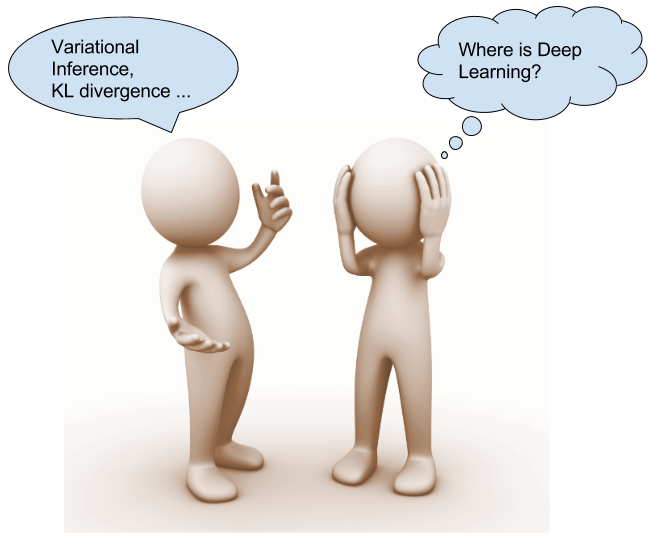
\includegraphics[width=0.7\textwidth]{where_is_deep_learning}
%         \label{fig:where_is_deep_learning}
%     \end{figure}
%     Image taken from Google Images (modified)
% \end{frame}onvergence Autoencodershi
% \begin{frame}{Connection with autoencoders}
%     \begin{itemize}
%         \item{
%             Lower bound is
%             $$\LB{}{\bxi} = \Exp{\qPhi(\bz|\bxi)}{- \log \qPhi(\bz|\bxi) + \log \pT(\bxi,\bz)}$$
%         }
%         \item{
%             This can also be written as
%             $$\LB{}{\bxi} = - D_{KL}(\qPhi(\bz|\bxi) || \pT(\bz)) + \Exp{\qPhi(\bz|\bxi)}{\log \pT(\bxi | \bz)}$$
%         }
%         \item {
%             First term is the distance of approximate posterior from the prior. Second term is expected negative reconstruction error.
%         }
%         \item {
%             Another estimator
%             \begin{align*}
%                 \LBT{B}{\bxi}
%                 &= - D_{KL}(\qPhi(\bz|\bxi) || \pT(\bz))
%                 + \frac{1}{L} \sum_{l=1}^L (\log \pT(\bxi|\bzil)) \\
%                 \text{where \quad} \bzil &= \gPhi(\bepsil,\bxi)
%                 \text{\quad and \quad} \bepsl \sim p(\beps)
%             \end{align*}
%         }
%         \item {
%             Useful when we can compute KL analytically. Reduces variance.
%         }
%     \end{itemize}

% \end{frame}




\section{Experiments and Results}


\begin{frame}{Variational Autoencoder}{Experiments and Results}
    \begin{itemize}
        \item {
            Experiments on MNIST and FRAY face dataset
        }
        \item {
            Metric
            \begin{itemize}
                \item{
                    Likelihood lower bound, same as optimization objective.
                }
            \end{itemize}
        }
    \end{itemize}
    \begin{figure}
        \centering
        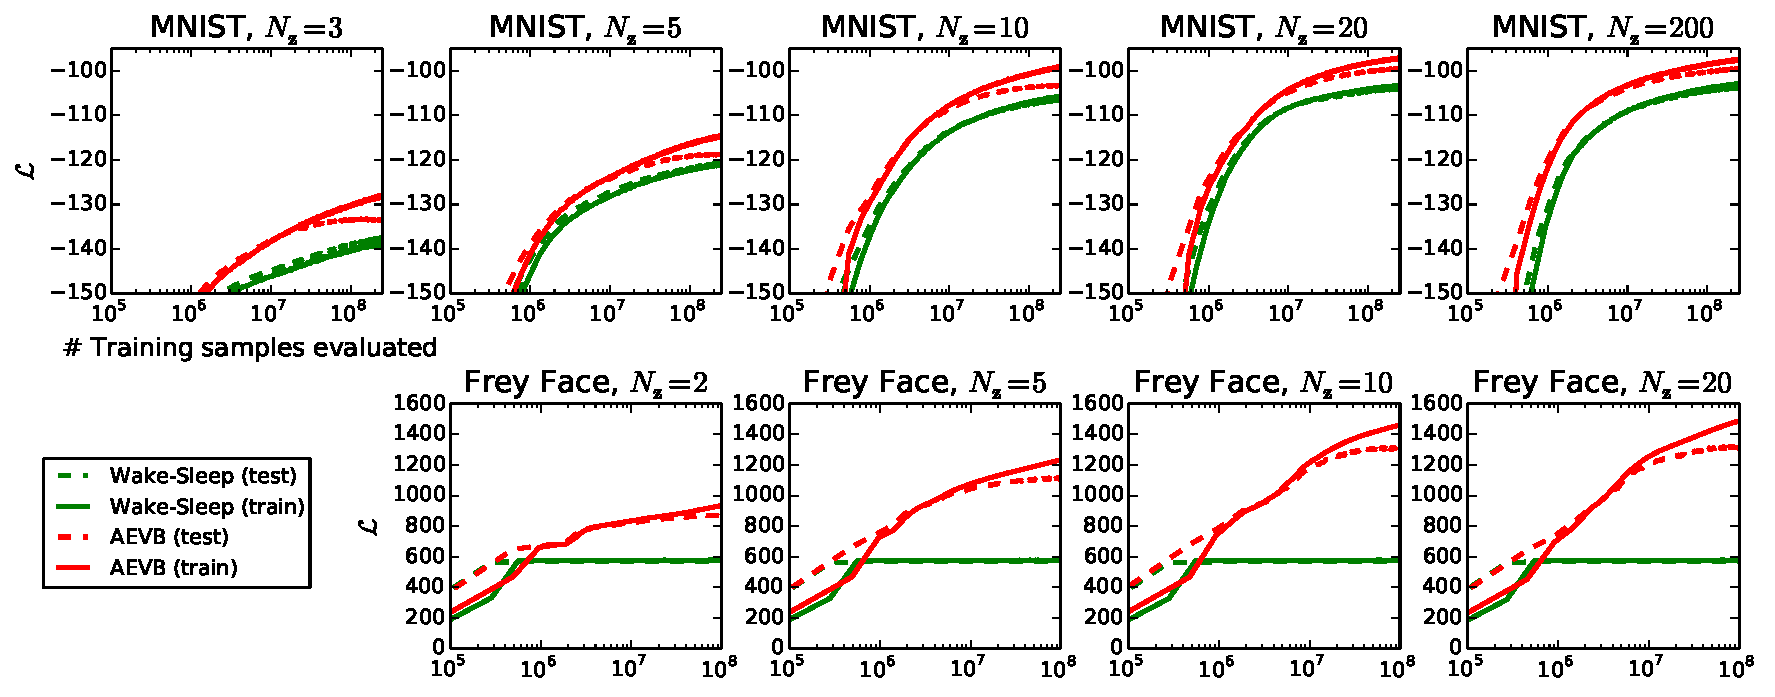
\includegraphics[width=0.8\textwidth]{graph_lowbound}
    \end{figure}
    {\small Image from https://arxiv.org/abs/1312.6114}
\end{frame}

\begin{frame}{Variational Autoencoder}{Experiments and Results}
    \begin{itemize}
        \item {
            Experiments on MNIST and FRAY face dataset
        }
        \item {
            Metric
            \begin{itemize}
                \item{
                    Estimated Marginal Likelihood
                }
            \end{itemize}
        }
    \end{itemize}
    \begin{figure}
        \centering
        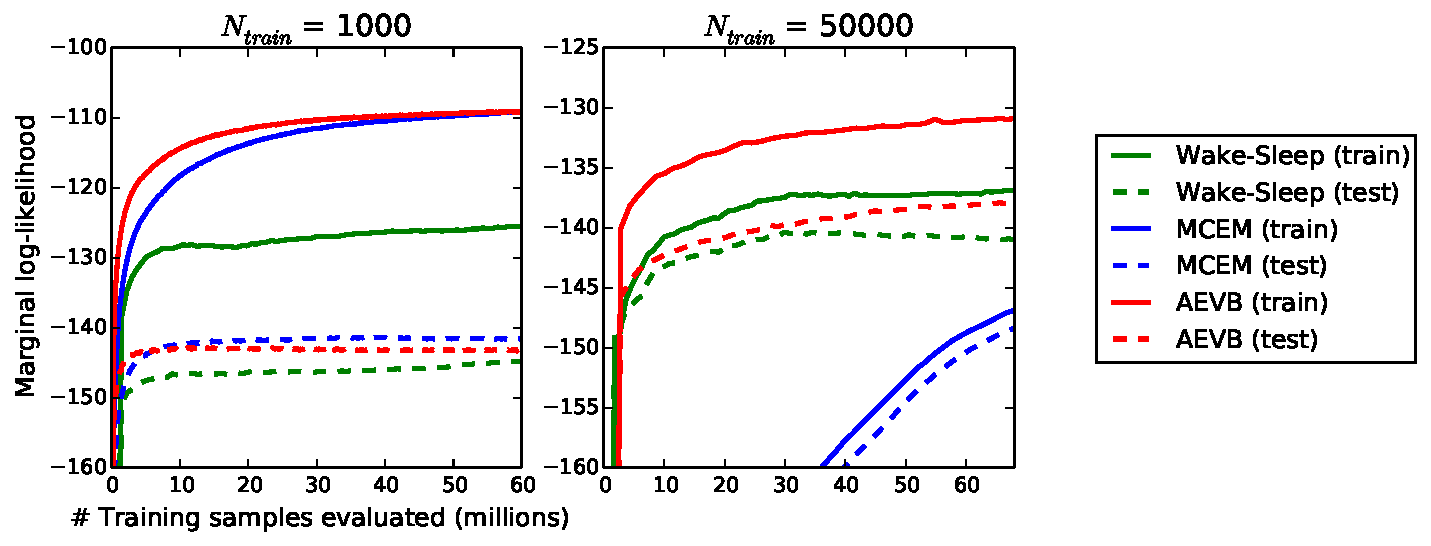
\includegraphics[width=0.8\textwidth]{graph_marglik}
    \end{figure}
    {\small Image from https://arxiv.org/abs/1312.6114}
\end{frame}


\begin{frame}{Variational Autoencoder}{Generated Samples}
    \begin{figure}
        \centering
        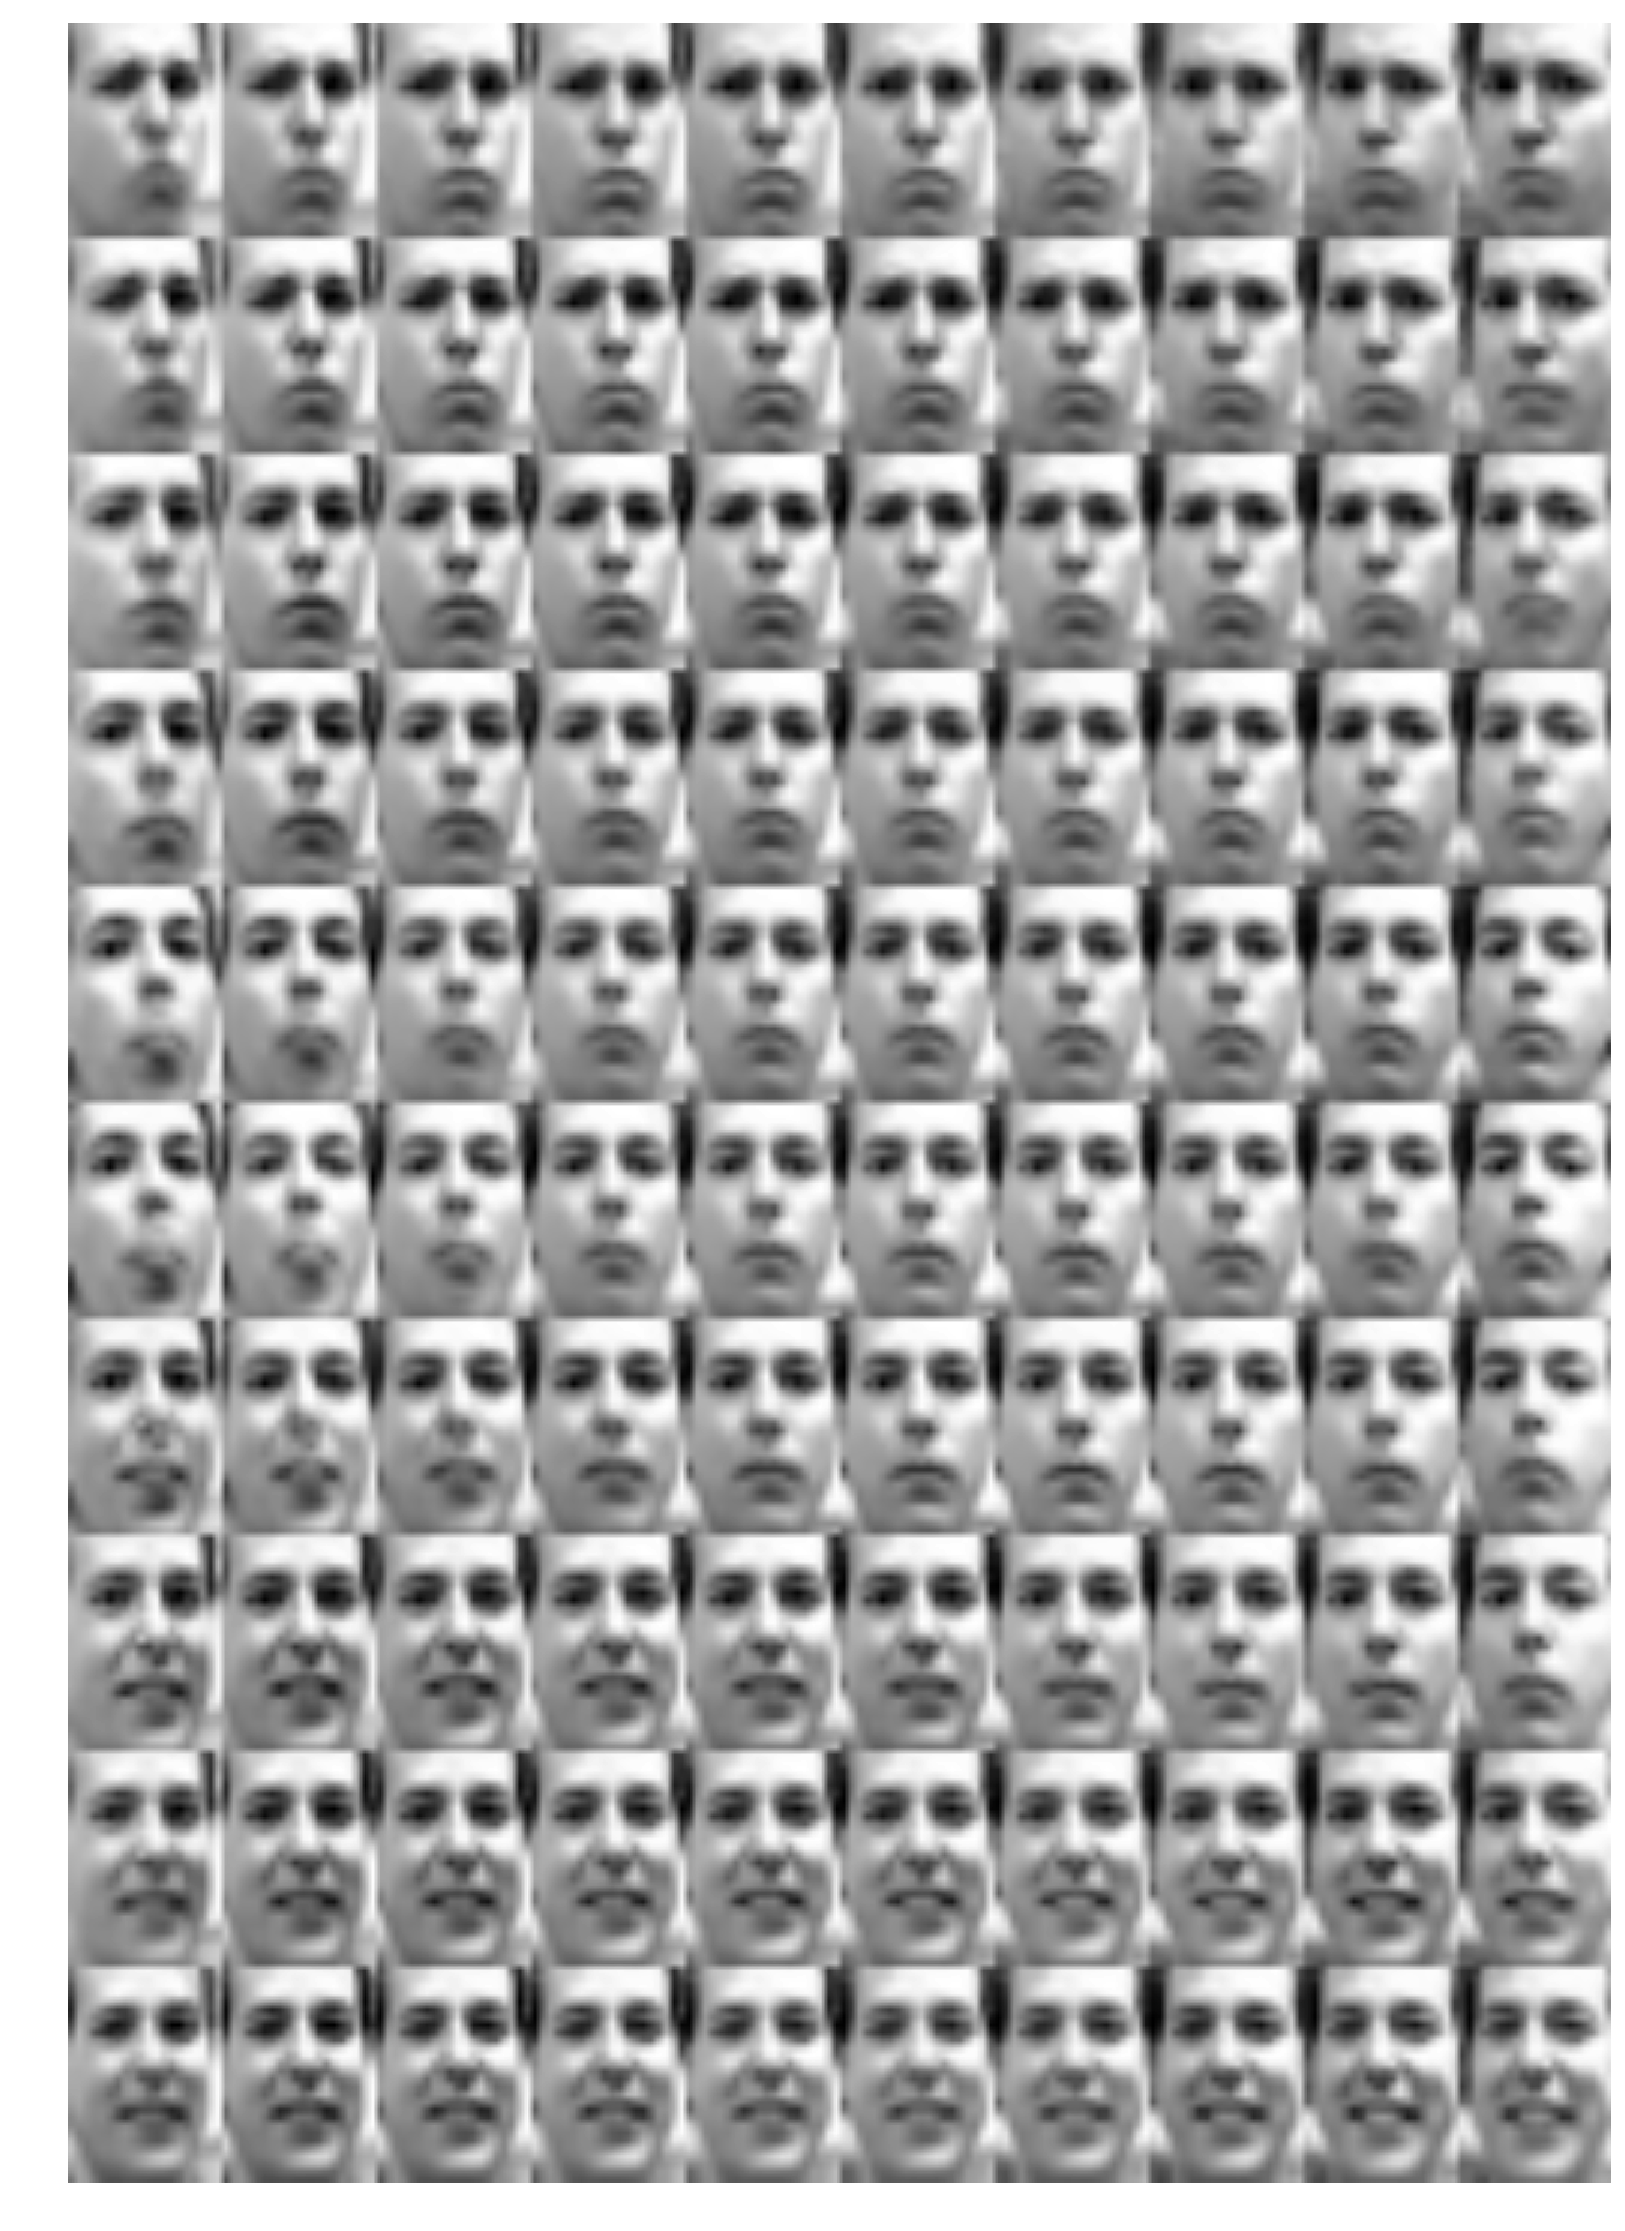
\includegraphics[height=0.6\textheight]{freyface_10x10}
        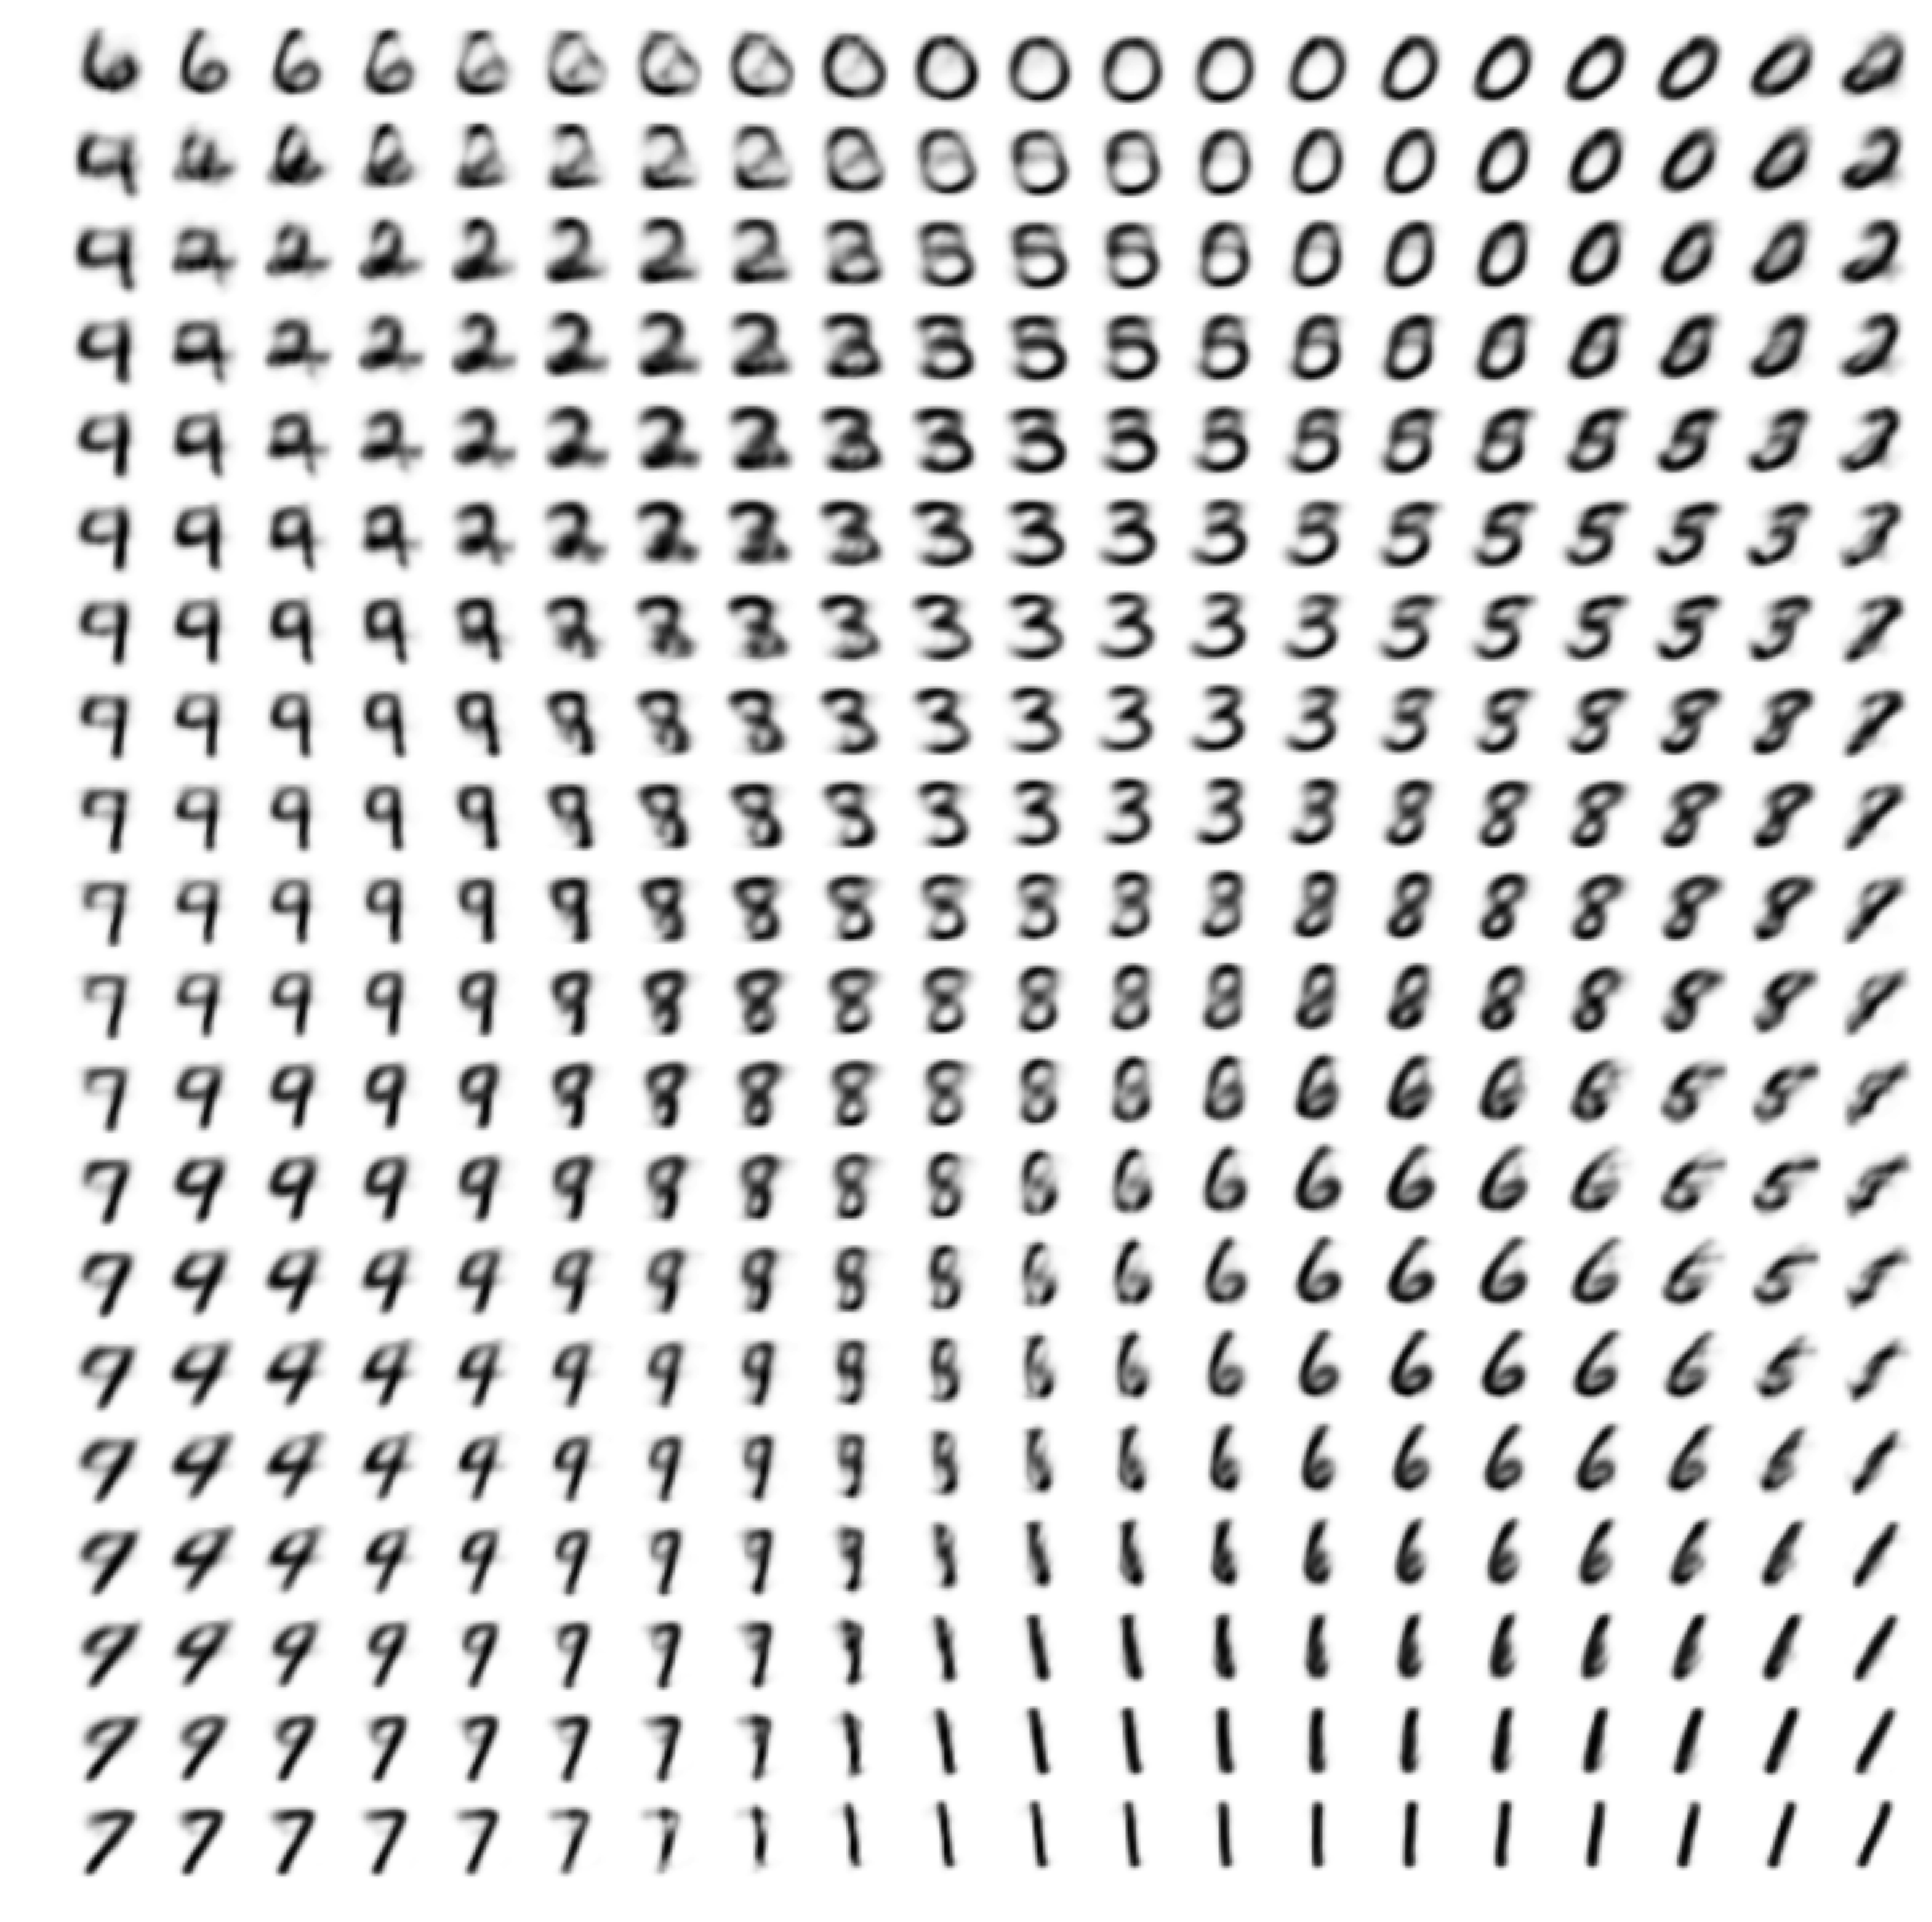
\includegraphics[height=0.6\textheight]{mnist_20x20}
    \end{figure}
    {\small Images from https://arxiv.org/abs/1312.6114}
\end{frame}

\begin{frame}{Variational Autoencoder}{Generated Samples}
    \begin{figure}
        \centering
        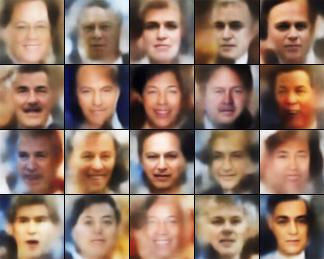
\includegraphics[height=0.7\textheight]{vae_faces}
    \end{figure}
    {\small Image from http://torch.ch/blog/2015/11/13/gan.html}
\end{frame}

\section{Demo}

\begin{frame}{MNIST VAE Demo}
    \url{https://transcranial.github.io/keras-js}
\end{frame}

\begin{frame}{Summary}
    \begin{itemize}
        \item {
            Problem : Latent variable model with intractable posterior, large dataset
        }
        \item {
            Solution
            \begin{itemize}
                \item Variational approximation for posterior
                \item Optimize variational lower bound
                \item Reparametrize recognition model to reduce variance
                \item Can plug in any function approximator (e.g. neural network)
            \end{itemize}
        }
        \item {Example application
            \begin{itemize}
                \item Variational Autoencoder
            \end{itemize}
        }
    \end{itemize}
\end{frame}

\begin{frame}{Discussion points}

    \begin{itemize}
        \item What are the limitations of VAEs?
        \item How do they compare to GANs?
        \item VAE output images more blurred as compared to GANs
        \item Other questions?
    \end{itemize}

    \vspace{3mm}
    \centering
    {\Huge Thanks!}

\end{frame}

\end{document}
